% 0122
\section{Single-Stream Transformer Architecture}
\label{appendix: Single-Stream Transformer Architecture}

In our research, we adopt the emerging single-stream diffusion transformer as our foundational architecture. This paradigm, exemplified by recent state-of-the-art open-source models Z-Image Turbo~\cite{zimage} and HunyuanImage-3.0~\cite{hunyuanimage3}, represents a radical departure from the architectural conventions of both SD v1.x~\cite{sd} and the recent Flux series~\cite{flux1kontext}.

As highlighted in Section~\ref{sec:motivation}, the evolution of T2I architectures has progressively moved towards higher modality fusion. SD v1.x models utilize a \emph{U-Net backbone} where visual features are processed in a dedicated path, and textual information is injected via distinct cross-attention layers. This separation allows for easy localization of concept-specific parameters. Flux introduces a \emph{dual-stream backbone} where text and image tokens are processed by separate weights ($\mathbf{W}_{txt}$ and $\mathbf{W}_{img}$) for the first half of the network before being concatenated. While more unified than SD v1.x, it still maintains explicit separation in the early stages.

In contrast, the pure single-stream architecture (as shown in Fig.~\ref{fig:architecture}) abolishes these boundaries entirely. As depicted in the diagram, text embeddings (from large language models or vision language models) and image patches (from VAE latents) are mapped into a common embedding space via linear projections. Crucially, they are concatenated into a \emph{Unified Input Sequence} before entering the transformer blocks. Within these blocks, the self-attention mechanism operates on this mixed sequence using \emph{shared} projection weights ($\mathbf{W}_{Q}$, $\mathbf{W}_{K}$, $\mathbf{W}_{V}$) for both modalities.
\begin{figure}[h]
	\centering
	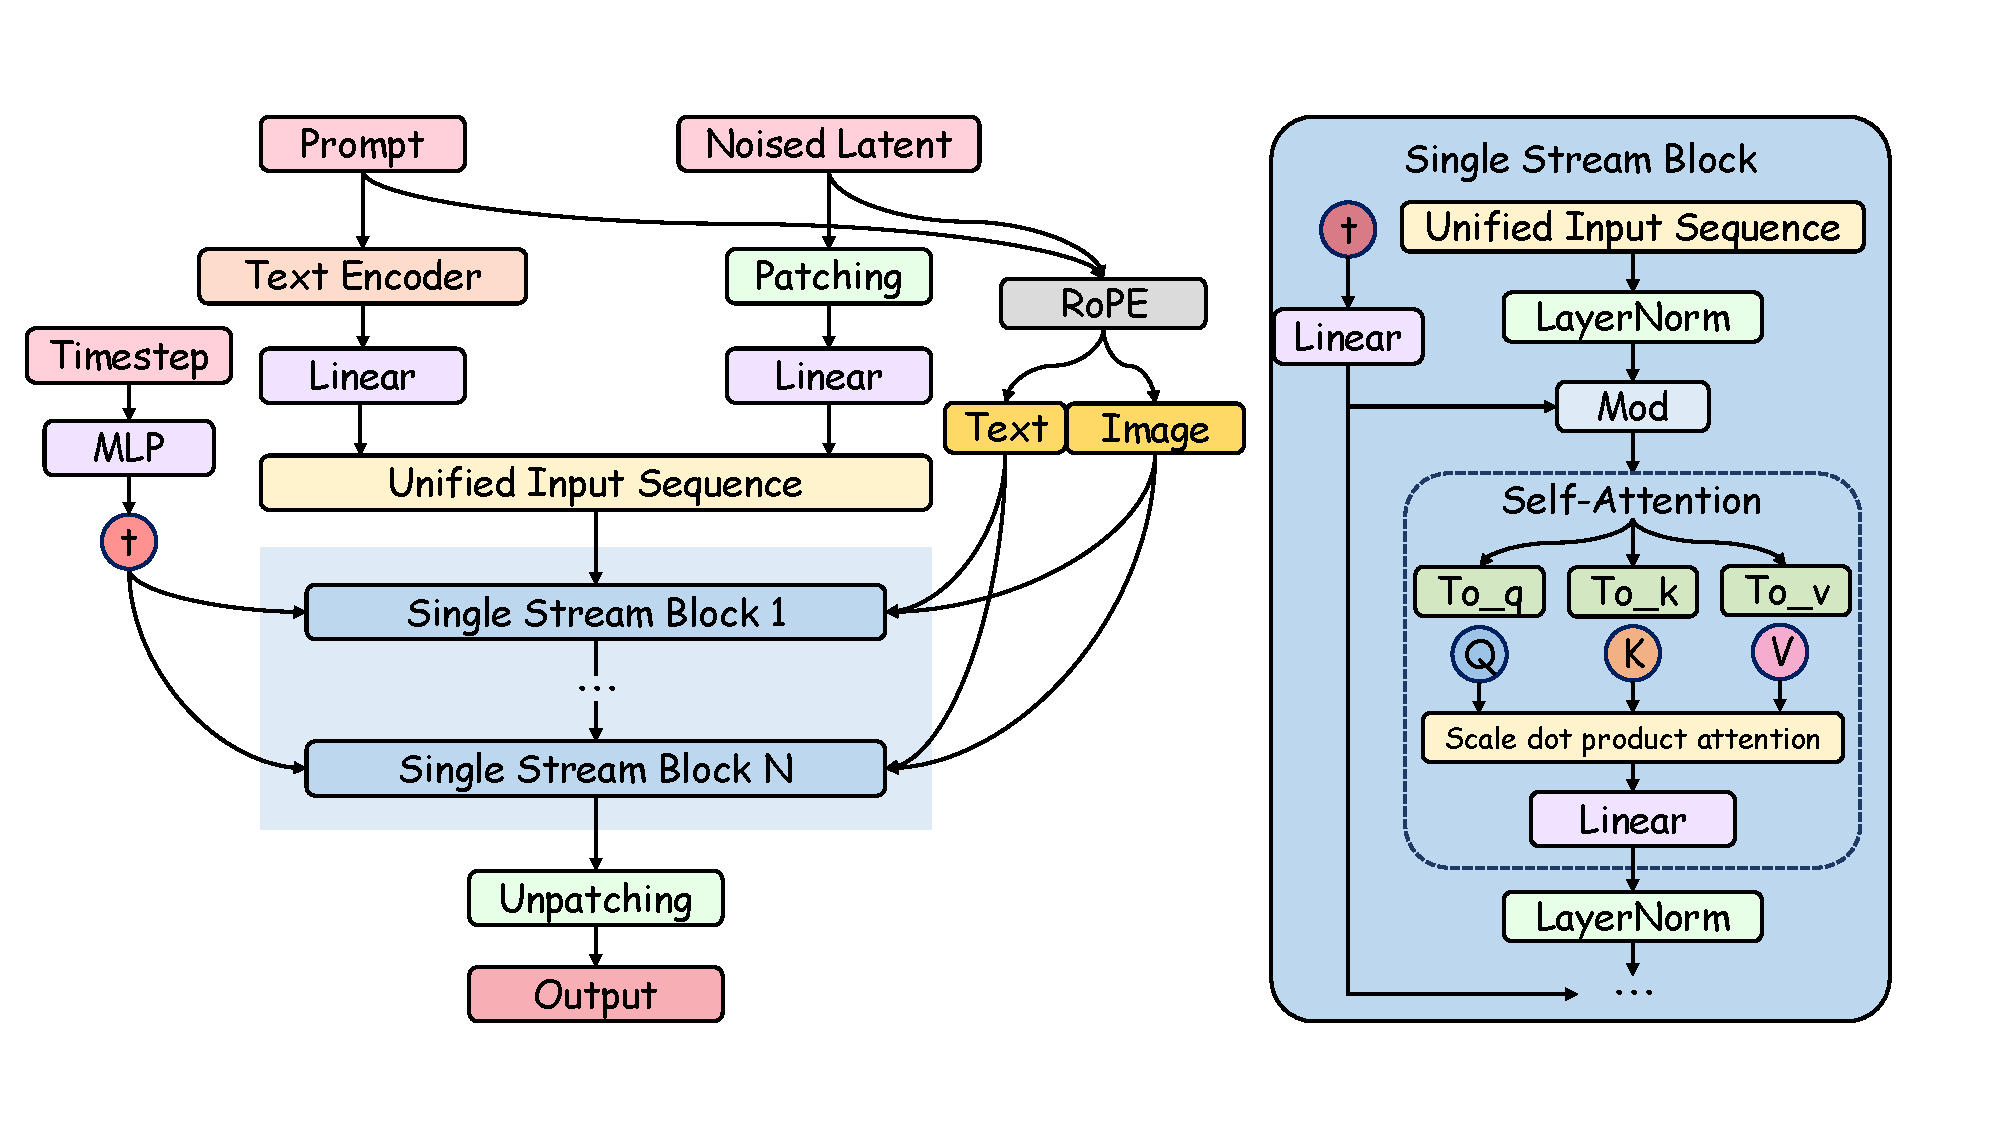
\includegraphics[width=1\linewidth]{fig/architecture.pdf}
    \vspace{5pt}
    \caption{\textbf{Abstract illustration of the Single-Stream DiT architecture.} The workflow begins with two parallel pathways: the prompt is processed by a text encoder, while the image latent is patched and projected similarly. These tokens are concatenated into a \emph{Unified Input Sequence}, which serves as the input to a stack of $N$ \emph{Single Stream Blocks}. Global conditioning information (\textit{e.g.}, Timestep) is injected into each block, influencing the layer normalization and attention scaling. Inside a Single Stream Block, the core \emph{Self-Attention} mechanism processes the sequence using shared Query ($Q$), Key ($K$), and Value ($V$) projections for both text and image tokens.}
    \label{fig:architecture}
\end{figure}

This ``Grand Unification" means that differentiation between text and image processing is no longer structural but semantic, driven solely by the token embeddings themselves. While this design maximizes parameter efficiency and generative quality, it introduces the \emph{entanglement} challenge we solve in Z-Erase: modifying weights to erase a text concept inherently risks corrupting the shared image generation mechanics.


% 0116
\section{Derivation Details of Lagrangian-Guided Adaptive Erasure Modulation}


In this section, we present the complete derivations and proofs that are omitted from the main text due to space limitations.


\subsection{Derivation of the dual problem}
\label{appendix: Derivation of the dual problem}

% 0121
To begin with, recall that the primal update in Eq.~\ref{eq: our goal} jointly optimizes a high-dimensional descent direction $\mathbf{d}_t$ while enforcing a preservation constraint through an inner product term:
\begin{equation}
    \max_{\mathbf{d}_t} \nabla \mathcal{L}_{er}(\theta_t) \cdot \mathbf{d}_t - \frac{1}{2}\|\mathbf{d}_t\|^2 
    , \,\,
    \text{s.t.} \nabla \mathcal{L}_{pr}(\theta_t) \cdot \mathbf{d}_t \ge -\varepsilon,
\end{equation}
Directly solving the primal form is undesirable for two reasons. First, the constraint only depends on the projection of $\mathbf{d}_t$ onto $\nabla \mathcal{L}_{pr}$, yet the optimization is carried out in the full parameter space, which obscures the proximal trade-off between erasure and preservation and offers no explicit control over the constraint (\textit{e.g.}, $\varepsilon$). Second, similar constrained gradient formulations in robust optimization and adversarial training~\cite{sener2019multitasklearningmultiobjectiveoptimization, yu2020gradientsurgerymultitasklearning, eupmu} have shown that converting the primal into its dual leads to substantially more stable updates and interpretable balancing coefficients. Motivated by these observations, we follow the standard primal-dual approach and rewrite Eq.~\ref{eq: our goal} into its dual form via a Lagrangian relaxation. This reparameterizes the update using a scalar dual variable $\lambda_t \ge 0$ and naturally leads to the closed-form solution for $\mathbf{d}_t$ once the dual objective is minimized. We provide the complete derivation below.
\begin{proof}
We start by constructing the Lagrangian function associated with the primal problem. The Lagrangian can be written as:
\begin{equation}
    \mathcal{L}(\mathbf{d}_t, \lambda_t) = \nabla \mathcal{L}_{er}(\theta_t) \cdot \mathbf{d}_t - \frac{1}{2} \left\|\mathbf{d}_t\right\|^2 + \lambda_t \left(\varepsilon + \nabla \mathcal{L}_{pr}(\theta_t) \cdot \mathbf{d}_t\right),
\end{equation}
where $\lambda_t \geq 0$ is the Lagrange multiplier corresponding to the constraint in the primal problem.

To find the dual objective, we first need to minimize the Lagrangian \textit{w.r.t} $\mathbf{d}_t$. Taking the gradient of $\mathcal{L}(\mathbf{d}_t, \lambda_t)$ \textit{w.r.t} $\mathbf{d}_t$ and setting it to zero, we have:
\begin{equation}
    \nabla_{\mathbf{d}_t} \mathcal{L}(\mathbf{d}_t, \lambda_t) = \nabla \mathcal{L}_{er}(\theta_t) + \lambda_t \nabla \mathcal{L}_{pr}(\theta_t) - \mathbf{d}_t = 0.
\end{equation}
Solving for $\mathbf{d}_t$, we obtain:
\begin{equation}
    \mathbf{d}_t = \nabla \mathcal{L}_{er}(\theta_t) + \lambda_t \nabla \mathcal{L}_{pr}(\theta_t).
\end{equation}
Substituting this back into the Lagrangian, we then get the dual function:
\begin{equation}
    \mathcal{L}_t(\lambda_t) = \mathcal{L}(\mathbf{d}_t, \lambda_t) = \nabla \mathcal{L}_{er}(\theta_t) \cdot (\nabla \mathcal{L}_{er}(\theta_t) + \lambda_t \nabla \mathcal{L}_{pr}(\theta_t)) - \frac{1}{2} \left\|\nabla \mathcal{L}_{er}(\theta_t) + \lambda_t \nabla \mathcal{L}_{pr}(\theta_t)\right\|^2 + \lambda_t \varepsilon.
\end{equation}
By expanding and simplifying, the dual objective finally becomes:
\begin{equation}
    \mathcal{L}_{t}(\lambda_t) =  \frac12 \big\| \nabla \mathcal L_{er}(\theta_t) + \lambda_t \nabla \mathcal L_{pr}(\theta_t) \big\|^2 + \lambda_t \varepsilon,
\end{equation}
which is the dual objective in Eq.~\ref{eq: dual problem}.
\end{proof}



\subsection{Derivation of the closed-form solution for the optimal direction $\mathbf{d}^*_t$}
\label{appendix: Derivation of the closed-form solution for the optimal direction}
\begin{proof}

To find the closed-form solution for the optimal direction $\mathbf{d}^*_t$, we first minimize the dual objective $\mathcal{L}_{t}(\lambda_t)$ \textit{w.r.t} $\lambda_t$. Taking the derivative of $\mathcal{L}_{t}(\lambda_t)$ \textit{w.r.t} $\lambda_t$ and setting it to zero, we then get:
\begin{equation}
    \label{eq: Taking the derivative of Lt wrt lambda t and setting it to zero}
    \frac{\partial \mathcal{L}_{t}(\lambda_t)}{\partial \lambda_t} = \nabla \mathcal{L}_{pr}(\theta_t) \cdot (\nabla \mathcal{L}_{er}(\theta_t) + \lambda_t \nabla \mathcal{L}_{pr}(\theta_t)) + \varepsilon = 0.
\end{equation}
Solving for $\lambda_t$, we obtain:
\begin{equation}
    \lambda_t^* = \frac{-\nabla \mathcal{L}_{pr}(\theta_t) \cdot \nabla \mathcal{L}_{er}(\theta_t) - \varepsilon}{\left\|\nabla \mathcal{L}_{pr}(\theta_t)\right\|^2}.
\end{equation}
Substituting $\lambda_t^*$ back into the expression for $\mathbf{d}^*_t$, we find the optimal update direction $\mathbf{d}^*_t$ as:
\begin{equation}
    \mathbf{d}^*_t = \begin{cases} 
\nabla \mathcal{L}_{er}(\theta_t) + \lambda^*_t \nabla \mathcal{L}_{pr}(\theta_t), & \text{if } \lambda_t^* > 0, \\
\nabla \mathcal{L}_{er}(\theta_t), & \text{if } \lambda_t^* \leq 0.
\end{cases}
\end{equation}
This is the closed-form solution for $\mathbf{d}^*_t$ stated in Eq.~\ref{eq: dt closed-form solution}.
\end{proof}


\subsection{Derivation of upper bound on preservation degradation}
\label{appendix: Derivation of upper bound on preservation degradation}
\begin{proof}
We first assume that the preservation loss $\mathcal{L}_{pr}$ is $\mathbf{G}$-smooth, meaning that its gradient is $\mathbf{G}$-Lipschitz:
\begin{equation}
\|\nabla \mathcal{L}_{pr}(\theta) - \nabla \mathcal{L}_{pr}(\theta')\| \le \mathbf{G}\|\theta-\theta'\|,
\end{equation}
for some constant $\mathbf{G} > 0$. By the standard smoothness inequality, we obtain:
\begin{equation}
    \mathcal{L}_{pr}(\theta_{t+1}) \le \mathcal{L}_{pr}(\theta_t) + \nabla \mathcal{L}_{pr}(\theta_t) ( \theta_{t+1}-\theta_t ) + \frac{\mathbf{G}}{2}\|\theta_{t+1}-\theta_t\|^2.
\end{equation}
Substituting $\theta_{t+1} = \theta_t - \alpha \mathbf{d}_t$ (where $\alpha$ is the learning rate of $\theta$) gives:
\begin{equation}
    \mathcal{L}_{pr}(\theta_{t+1}) - \mathcal{L}_{pr}(\theta_t) \le -\alpha \nabla \mathcal{L}_{pr}(\theta_t) \mathbf{d}_t + \frac{\mathbf{G}\alpha^2}{2}\|\mathbf{d}_t\|^2.
\end{equation}
Using the primal constraint $\nabla \mathcal{L}_{pr}(\theta_t) \cdot \mathbf{d}_t \ge -\varepsilon$, we obtain:
\begin{equation}
    \mathcal{L}_{pr}(\theta_{t+1}) - \mathcal{L}_{pr}(\theta_t) \le \alpha \varepsilon + \frac{\mathbf{G}\alpha^2}{2}\|\mathbf{d}_t\|^2 \lesssim \alpha \varepsilon,
\end{equation}
where the final approximation holds when $\alpha$ is sufficiently small such that the quadratic term becomes negligible. Summing over $0$ to $t$, we get:
\begin{equation}
    \mathcal{L}_{pr}(\theta_t)-\mathcal{L}_{pr}(\theta_0) \;\lesssim\; \mathcal{O}(t\,\varepsilon\,\alpha),
\end{equation}
which is the upper bound in Eq.~\ref{eq: Lpr is bounded by}.
\end{proof}


\section{Convergence Analysis of Lagrangian-Guided Adaptive Erasure Modulation}
\label{appendix: Convergence Analysis of Constraint-Aware Dynamic Balancing}

In this section, we provide a theoretical analysis of the convergence properties of the proposed \textbf{Lagrangian-Guided Adaptive Erasure Modulation} algorithm. Our primary goal is to demonstrate that Algorithm~\ref{alg:z-erase}, despite employing a specific first-order Taylor approximation for computational efficiency (Eq.~\ref{first-order Taylor expansion}), successfully converges to a \textbf{Pareto stationary point}. This implies that the algorithm finds a solution where the erasure objective $\mathcal{L}_{er}$ cannot be further optimized without violating the preservation constraint defined by $\mathcal{L}_{pr}$ and tolerance $\varepsilon$.

Formally, the optimization problem in Z-Erase can be modeled as a constrained optimization problem: $\min_{\theta} \mathcal{L}_{er}(\theta)$ s.t. the preservation degradation is bounded by $\varepsilon$. Our algorithm solves this via a dynamic Lagrangian method. The core challenge in the analysis lies in the coupled dynamics of the model parameters $\theta_t$ and the constraint weight $\lambda_t$, particularly given that $\lambda_t$ is updated via an \textbf{implicit approximation} (without calculating the full Hessian or second-order information).

To rigorously prove the convergence, our analysis proceeds in three main steps:
\begin{enumerate}
    \item \textbf{Approximation Bound}: We first establish that the implicitly estimated gradient for updating $\lambda_t$ (derived from the loss difference in Eq.~\ref{first-order Taylor expansion}) serves as a valid proxy for the true gradient, with the error bounded by the learning rate $\alpha$.
    \item \textbf{Dynamic Regret Analysis}: We treat the update of the dynamic weight $\lambda_t$ as an online learning process. By leveraging results from Online Gradient Descent (OGD), we prove that the accumulation of errors (regret) due to the dynamic nature of $\lambda_t$ and $\beta$ is sub-linear and controllable. This answers why the dynamic variation of $\beta$ (or $\lambda$) does not prevent the system from settling.
    \item \textbf{Convergence to Stationarity}: Finally, combining the smoothness of the objective functions and the bounded regret, we prove that the gradient of the total objective tends to zero, ensuring the method converges to a valid stationary solution.
\end{enumerate}

\subsection{Approximation bound}

Our analysis relies on the following standard assumptions regarding the erasure objective $\mathcal{L}_{er}$ and the preservation objective $\mathcal{L}_{pr}$.

\begin{assumption}[Boundedness and Lipschitz Continuity]
\label{assum:lipschitz}
For both objective functions $f \in \{\mathcal{L}_{er}, \mathcal{L}_{pr}\}$, we assume they are bounded below and $\mathbf{L}$-Lipschitz continuous. That is, for any parameters $\theta_1, \theta_2$, there exists a constant $\mathbf{L} > 0$ such that $\|\nabla f(\theta_1)\| \le \mathbf{L}$ and $|f(\theta_1) - f(\theta_2)| \le \mathbf{L} \|\theta_1 - \theta_2\|$.
\end{assumption}

\begin{assumption}[$\mathbf{G}$-Smoothness]
\label{assum:smoothness}
The objective functions are differentiable and their gradients are $\mathbf{G}$-Lipschitz continuous ($\mathbf{G}$-Smooth). Specifically, there exists a constant $\mathbf{G} > 0$ such that:
\begin{equation}
    \|\nabla f(\theta_1) - \nabla f(\theta_2)\| \le \mathbf{G} \|\theta_1 - \theta_2\|.
\end{equation}
A key consequence of $\mathbf{G}$-smoothness is the descent lemma (or quadratic upper bound):
\begin{equation}
    |f(\theta_2) - f(\theta_1) - \nabla f(\theta_1)^\top (\theta_2 - \theta_1)| \le \frac{\mathbf{G}}{2} \|\theta_2 - \theta_1\|^2.
\end{equation}
\end{assumption}

Recall that the core of our \textbf{Lagrangian-Guided Adaptive Erasure Modulation} involves solving the dual problem (Eq.~\ref{eq: dual problem}) with respect to $\lambda_t$. The update rule for $\lambda_t$ depends on the gradient of the dual objective $\mathcal{L}_t(\lambda_t)$.
From Eq.~\ref{eq: Taking the derivative of Lt wrt lambda t and setting it to zero} (in the preceding derivation), the \emph{true gradient} of the dual objective \textit{w.r.t} $\lambda_t$ is given by:
\begin{equation}
    g_t \triangleq \nabla_{\lambda_t} \mathcal{L}_t(\lambda_t) = \nabla \mathcal{L}_{pr}(\theta_t) \cdot \mathbf{d}_t + \varepsilon,
\end{equation}
where $\mathbf{d}_t$ is the update direction for model parameters.
However, computing $\nabla \mathcal{L}_{pr}(\theta_t) \cdot \mathbf{d}_t$ exactly requires two backward passes. To improve efficiency, Z-Erase utilizes an \textbf{approximate gradient} update (Eq.~\ref{first-order Taylor expansion}) using the loss difference from the first-order Taylor approximation:
\begin{equation}
    \tilde{g}_t \triangleq \frac{1}{\alpha} (\mathcal{L}_{pr}(\theta_{t-1}) - \mathcal{L}_{pr}(\theta_{t})) + \varepsilon,
\end{equation}
where $\theta_{t} = \theta_{t-1} - \alpha \mathbf{d}_{t-1}$.

The following lemma establishes that this implicit approximation is a theoretically valid proxy, as the approximation error is bounded by the model learning rate $\alpha$.

\begin{lemma}[Approximation Error Bound]
\label{lemma:approx_error}
Under Assumptions \ref{assum:lipschitz} and \ref{assum:smoothness}, the difference between the true gradient $g_t$ and the approximate gradient $\tilde{g}_t$ used in Algorithm 1 is bounded by the step size $\alpha$:
\begin{equation}
    \| \tilde{g}_t - g_t \| \le \frac{\mathbf{G} \alpha}{2} \|\mathbf{d}_{t-1}\|^2 \le \mathcal{O}(\alpha).
\end{equation}
\end{lemma}

\begin{proof}
Substituting the parameter update rule $\theta_{t} = \theta_{t-1} - \alpha \mathbf{d}_{t-1}$ into the smoothness inequality (Assumption \ref{assum:smoothness}) for the preservation loss $\mathcal{L}_{pr}$, we have:
\begin{equation}
    \mathcal{L}_{pr}(\theta_{t}) \le \mathcal{L}_{pr}(\theta_{t-1}) + \nabla \mathcal{L}_{pr}(\theta_{t-1})^\top (-\alpha \mathbf{d}_{t-1}) + \frac{\mathbf{G}}{2} \|-\alpha \mathbf{d}_{t-1}\|^2.
\end{equation}
Rearranging the terms to isolate the dot product $\nabla \mathcal{L}_{pr}(\theta_{t-1})^\top \mathbf{d}_{t-1}$:
\begin{equation}
    \alpha \nabla \mathcal{L}_{pr}(\theta_{t-1})^\top \mathbf{d}_{t-1} \le \mathcal{L}_{pr}(\theta_{t-1}) - \mathcal{L}_{pr}(\theta_{t}) + \frac{\mathbf{G} \alpha^2}{2} \|\mathbf{d}_{t-1}\|^2.
\end{equation}
Similarly, using the lower bound property of smoothness, we can obtain:
\begin{equation}
    \mathcal{L}_{pr}(\theta_{t}) \ge \mathcal{L}_{pr}(\theta_{t-1}) - \alpha \nabla \mathcal{L}_{pr}(\theta_{t-1})^\top \mathbf{d}_{t-1} - \frac{\mathbf{G} \alpha^2}{2} \|\mathbf{d}_{t-1}\|^2,
\end{equation}
which implies:
\begin{equation}
    \alpha \nabla \mathcal{L}_{pr}(\theta_{t-1})^\top \mathbf{d}_{t-1} \ge \mathcal{L}_{pr}(\theta_{t-1}) - \mathcal{L}_{pr}(\theta_{t}) - \frac{\mathbf{G} \alpha^2}{2} \|\mathbf{d}_{t-1}\|^2.
\end{equation}
Combining these two inequalities, the absolute difference satisfies:
\begin{equation}
    \left| (\mathcal{L}_{pr}(\theta_{t-1}) - \mathcal{L}_{pr}(\theta_{t})) - \alpha \nabla \mathcal{L}_{pr}(\theta_{t-1})^\top \mathbf{d}_{t-1} \right| \le \frac{\mathbf{G} \alpha^2}{2} \|\mathbf{d}_{t-1}\|^2.
\end{equation}
Now, we explicitly compare the gradients. The error is:
\begin{align}
    \| \tilde{g}_t - g_t \| &= \left| \left( \frac{1}{\alpha} (\mathcal{L}_{pr}(\theta_{t-1}) - \mathcal{L}_{pr}(\theta_{t})) + \varepsilon \right) - \left( \nabla \mathcal{L}_{pr}(\theta_{t-1}) \cdot \mathbf{d}_{t-1} + \varepsilon \right) \right| \\
    &= \frac{1}{\alpha} \left| (\mathcal{L}_{pr}(\theta_{t-1}) - \mathcal{L}_{pr}(\theta_{t})) - \alpha \nabla \mathcal{L}_{pr}(\theta_{t-1}) \cdot \mathbf{d}_{t-1} \right| \\
    &\le \frac{1}{\alpha} \cdot \frac{\mathbf{G} \alpha^2}{2} \|\mathbf{d}_{t-1}\|^2 \\
    &= \frac{\mathbf{G} \alpha}{2} \|\mathbf{d}_{t-1}\|^2.
\end{align}
Since $\mathcal{L}_{er}$ and $\mathcal{L}_{pr}$ are Lipschitz continuous (Assumption \ref{assum:lipschitz}), the gradient $\nabla \mathcal{L}_{er}$ and $\nabla \mathcal{L}_{pr}$ are bounded, which implies the update direction $\mathbf{d}_t$ (a linear combination of gradients) is also bounded, \textit{i.e.}, $\|\mathbf{d}_{t-1}\|^2 \le C$. Thus, strictly speaking, $\| \tilde{g}_t - g_t \| \le \mathcal{O}(\alpha)$.
This concludes the proof that the implicit gradient approximation is asymptotically accurate as $\alpha \to 0$.
\end{proof}

\subsection{Dynamic regret analysis}
\label{sec:dynamic_regret}

Since the model parameters $\theta_t$ are updated at each step, the dual objective function $\mathcal{L}_t(\lambda)$ is actually time-varying. Consequently, the update of the constraint weight $\lambda_t$ via gradient ascent can be formulated as an Online Convex Optimization (OCO) problem. To prove convergence, we must bound the \textit{dynamic regret}, which measures the accumulated loss difference between our algorithm's choice of $\lambda_t$ and the sequence of optimal comparators $\lambda_t^*$.

We define the dual objective at step $t$ following Eq.~\ref{eq: dual problem} as $\mathcal{L}_t(\lambda_t) = \frac{1}{2}\|\nabla \mathcal{L}_{er}(\theta_t) + \lambda_t \nabla \mathcal{L}_{pr}(\theta_t)\|^2 + \lambda_t \varepsilon$. Note that we aim to minimize this dual objective \textit{w.r.t} $\lambda_t$.
The dynamic regret is defined as:
\begin{equation}
    \mathcal{R}_T \triangleq \sum_{t=1}^T \left( \mathcal{L}_t(\lambda_t) - \mathcal{L}_t(\lambda_t^*) \right),
\end{equation}
where $\lambda_t^* = \arg\min_{\lambda_t \ge 0} \mathcal{L}_t(\lambda_t)$ is the optimal dual variable at step $t$ (derived in Eq.~\ref{eq: lambda_t closed-form solution}).

To bound this regret, we first establish a bound on the \emph{total functional variation of the dual objective}, which quantifies how much the optimization landscape changes between steps.

\begin{lemma}[Total Functional Variation]
\label{lemma:func_variation}
Under Assumptions \ref{assum:lipschitz} and \ref{assum:smoothness}, let $D$ be the upper bound of the dual variable $\lambda$. The variation of the dual objective function between consecutive steps is bounded by the learning rate $\alpha$:
\begin{equation}
    \sum_{t=0}^{T-1} \sup_{\lambda \in [0, D]} | \mathcal{L}_{t+1}(\lambda) - \mathcal{L}_t(\lambda) | \le C_1 T \alpha,
\end{equation}
where $C_1$ is a constant depending on Lipschitz constant $\mathbf{L}$, Smoothness constant $\mathbf{G}$, and $D$.
\end{lemma}

\begin{proof}
For any $\lambda$, the variation is:
\begin{align}
    |\mathcal{L}_{t+1}(\lambda) - \mathcal{L}_t(\lambda)| &= \left| \frac{1}{2}\|\nabla \mathcal{L}_{er}(\theta_{t+1}) + \lambda \nabla \mathcal{L}_{pr}(\theta_{t+1})\|^2 - \frac{1}{2}\|\nabla \mathcal{L}_{er}(\theta_t) + \lambda \nabla \mathcal{L}_{pr}(\theta_t)\|^2 \right| \\
    &= \frac{1}{2} \left| \left( \mathbf{v}_{t+1} + \mathbf{v}_t \right)^\top \left( \mathbf{v}_{t+1} - \mathbf{v}_t \right) \right|,
\end{align}
where we denote the composite gradient vector $\mathbf{v}_t(\lambda) \triangleq \nabla \mathcal{L}_{er}(\theta_t) + \lambda \nabla \mathcal{L}_{pr}(\theta_t)$.
By L-Lipschitz continuity, $\|\mathbf{v}_t\| \le \mathcal{L}(1+\lambda)$. By $\mathbf{G}$-smoothness, $\|\mathbf{v}_{t+1} - \mathbf{v}_t\| \le \mathbf{G}(1+\lambda)\|\theta_{t+1} - \theta_t\| = \mathbf{G}(1+\lambda)\alpha \|\mathbf{d}_t\|$.
Substituting these bounds:
\begin{align}
    |\mathcal{L}_{t+1}(\lambda) - \mathcal{L}_t(\lambda)| &\le \frac{1}{2} \cdot 2\mathbf{L}(1+\lambda) \cdot \mathbf{G}(1+\lambda)\alpha \|\mathbf{d}_t\| \\
    &\le \alpha \cdot \mathbf{G} \mathbf{L} (1+D)^2 \|\mathbf{d}_t\|.
\end{align}
Since $\|\mathbf{d}_t\|$ is bounded (as gradients are bounded), let $C_1 = \mathbf{G} \mathbf{L} (1+D)^2 \max \|\mathbf{d}_t\|$. Summing over $t$ yields the lemma.
\end{proof}

With the variation bound established, we invoke the standard dynamic regret bound for Online Gradient Descent (OGD)~\cite{Onlineconvexprogramming, jadbabaie2015onlineoptimizationcompeting}.

\begin{theorem}[Dynamic Regret Bound]
\label{thm:dynamic_regret}
Suppose the updates for $\lambda_t$ follow the gradient descent rule with a fixed step size $\beta$ (as in Eq.~\ref{eq: iteratively update lambda t via gradient descent approximation}), and model updates use a fixed learning rate $\alpha$. Using the approximate gradient $\tilde{g}_t$ where $\|\tilde{g}_t - g_t\| \le \mathcal{O}(\alpha)$, the average dynamic regret is bounded by terms dependent on the step sizes and the horizon $T$:
\begin{equation}
    \frac{1}{T} \sum_{t=1}^T \left( \mathcal{L}_t(\lambda_t) - \mathcal{L}_t(\lambda_t^*) \right) \le \mathcal{O}\left(\frac{1}{\beta T}\right) + \mathcal{O}(\beta) + \mathcal{O}(\alpha).
\end{equation}
As $T \to \infty$, the average regret converges to a neighborhood $\mathcal{O}(\alpha + \beta)$ determined by the chosen hyperparameters.
\end{theorem}

\begin{proof}
(Sketch) The regret in online learning with inexact gradients can be decomposed into two components: one arising from the non-stationarity of the environment (tracking error) and one from the gradient approximation error.
Standard results in Online Convex Optimization (OCO) with \textit{constant step sizes} indicate that the tracking error is upper-bounded by $\mathcal{O}(\beta)$ (representing the system's reaction speed to dynamic changes) plus an initialization term decaying as $\mathcal{O}(\frac{1}{\beta T})$.
Additionally, Lemma \ref{lemma:approx_error} ensures that the gradient approximation error is bounded by $\mathcal{O}(\alpha)$ at each step.
Averaging over $T$ steps, the total regret bound becomes $\mathcal{O}(\frac{1}{\beta T} + \beta + \alpha)$.
This result provides sufficient theoretical justification for our practical implementation: while exact convergence to zero requires diminishing steps, establishing small fixed $\alpha$ and $\beta$ guarantees the system stabilizes within a tight, controlled neighborhood of the optimal Pareto front.
\end{proof}

\subsection{Convergence to Pareto stationarity}
With the dynamic regret bound established, we now prove the convergence of the model parameters $\theta$ to a stationary point. We construct a total composite objective function at each step $t$ defined by the dynamically tracked weight $\lambda_t$:
\begin{equation}
    \mathcal{J}_t(\theta) \triangleq \mathcal{L}_{er}(\theta) + \lambda_t \mathcal{L}_{pr}(\theta).
\end{equation}
Our goal is to show that the gradient of this composite objective vanishes, implying that the algorithm reaches a consistent solution.

\begin{theorem}[Pareto Stationarity]
\label{thm:stationarity}
Under Assumptions \ref{assum:lipschitz} and \ref{assum:smoothness}, and given the diminishing step sizes $\alpha, \beta$ satisfying the conditions in Theorem \ref{thm:dynamic_regret}, the sequence of iterates generated by Algorithm 1 satisfies:
\begin{equation}
    \lim_{T \to \infty} \min_{t=1,\dots,T} \|\nabla \mathcal{L}_{er}(\theta_t) + \lambda_t \nabla \mathcal{L}_{pr}(\theta_t) \|^2 = 0.
\end{equation}
\end{theorem}

\begin{proof}
Consider the update rule $\theta_{t+1} = \theta_t - \alpha_t \mathbf{d}_t$. By the construction of our algorithm (Eq.~\ref{eq: dt closed-form solution}), the update direction is the gradient of the Lagrangian:
\begin{equation}
    \mathbf{d}_t = \nabla \mathcal{L}_{er}(\theta_t) + \lambda_t \nabla \mathcal{L}_{pr}(\theta_t).
\end{equation}
Applying the $\mathbf{G}$-smoothness assumption to the composite function $\mathcal{J}_t(\theta)$ (noting that $\mathcal{J}_t$ is smooth since it is a linear combination of smooth functions):
\begin{align}
    \mathcal{J}_t(\theta_{t+1}) &\le \mathcal{J}_t(\theta_t) + \nabla \mathcal{J}_t(\theta_t)^\top (\theta_{t+1} - \theta_t) + \frac{\mathbf{G}(1+\lambda_t)}{2} \|\theta_{t+1} - \theta_t\|^2 \\
    &= \mathcal{J}_t(\theta_t) - \alpha \|\mathbf{d}_t\|^2 + \frac{\mathbf{G}(1+\lambda_t)\alpha_t^2}{2} \|\mathbf{d}_t\|^2 \\
    &= \mathcal{J}_t(\theta_t) - \alpha \left( 1 - \frac{\alpha \mathbf{G}(1+\lambda_t)}{2} \right) \|\mathbf{d}_t\|^2.
\end{align}
Since $\lambda_t$ is bounded (let $\lambda_t \le D$) and we choose a sufficiently small step size $\alpha < \frac{2}{\mathbf{G}(1+D)}$, the coefficient $\left( 1 - \frac{\alpha \mathbf{G}(1+\lambda_t)}{2} \right)$ is positive. Let this coefficient be $c > 0$. Rearranging the terms, we get:
\begin{equation}
    c \alpha \|\mathbf{d}_t\|^2 \le \mathcal{J}_t(\theta_t) - \mathcal{J}_t(\theta_{t+1}).
\end{equation}
However, unlike standard SGD, our objective $\mathcal{J}_t$ changes at each step because $\lambda_t$ updates to $\lambda_{t+1}$. We decompose the total variation:
\begin{align}
    \mathcal{J}_{t+1}(\theta_{t+1}) - \mathcal{J}_t(\theta_t) &= \underbrace{\mathcal{J}_{t+1}(\theta_{t+1}) - \mathcal{J}_t(\theta_{t+1})}_{\text{due to } \lambda \text{ update}} + \underbrace{\mathcal{J}_t(\theta_{t+1}) - \mathcal{J}_t(\theta_t)}_{\text{due to } \theta \text{ update}} \\
    &= (\lambda_{t+1} - \lambda_t)\mathcal{L}_{pr}(\theta_{t+1}) + (\mathcal{J}_t(\theta_{t+1}) - \mathcal{J}_t(\theta_t)).
\end{align}
Summing from $t=1$ to $T$:
\begin{equation}
    \sum_{t=1}^T c \alpha \|\mathbf{d}_t\|^2 \le \mathcal{J}_1(\theta_1) - \mathcal{J}_{T+1}(\theta_{T+1}) + \sum_{t=1}^T (\lambda_{t+1} - \lambda_t)\mathcal{L}_{pr}(\theta_{t+1}).
\end{equation}
Standard telescope sum analysis combined with the bounded variation of $\lambda$ (from Theorem \ref{thm:dynamic_regret}) ensures the right side is bounded by a constant $C_2$.
Therefore, $\sum_{t=1}^T \alpha_t \|\mathbf{d}_t\|^2 \le C_2 < \infty$. Given that $\sum \alpha \to \infty$ (for standard decay rates), it implies that $\liminf_{t \to \infty} \|\mathbf{d}_t\|^2$ must be 0.
Specifically, for standard choices of $\alpha$, we have:
\begin{equation}
    \min_{t=1,\dots,T} \|\mathbf{d}_t\|^2 \le \frac{C_2}{\sum_{t=1}^T \alpha} \xrightarrow{T \to \infty} 0.
\end{equation}
This proves that the algorithm converges to a point where the update direction $\mathbf{d}_t$ vanishes. Recall that $\mathbf{d}_t$ is the gradient of the Lagrangian. $\mathbf{d}_t = 0$ implies the KKT condition for stationarity is satisfied for the constrained optimization problem.
\end{proof}

\paragraph{Remark on Hyperparameters.}
The theoretical analysis above assumes diminishing step sizes $\alpha, \beta$ to guarantee asymptotic convergence. In our practical implementation (Section~\ref{sec: Implementation Details}), we adopt fixed hyperparameters ($\alpha=0.001$, $\beta=0.1$) for finite-step training. As indicated by Theorem \ref{thm:dynamic_regret}, the stationary error is bounded by terms related to the step sizes. A small, fixed step size effectively maintains the system within a small neighborhood of the optimal Pareto front, balancing convergence speed and stability in the non-convex landscape of diffusion models.



\section{Additional Implementation Details and Results}
\label{appendix: Additional Experimental Details and Results}

\subsection{Hyperparameter settings for $\varepsilon$ across experiments}
The tolerance parameter $\varepsilon$ controls how tightly the preservation constraint is enforced and directly determines the trade-off between erasing the target concept and maintaining the model's overall utility. Small values of $\varepsilon$ restrict the update direction and prioritize preservation, which is preferable for fragile concepts or datasets with high semantic entanglement. Larger values relax the constraint and enable more aggressive erasure at the cost of controlled performance drift. In all our experiments we find that $\varepsilon$ is robust within a moderate range (typically $10^{-3}$–$10^{-1}$), and does not require fine-grained tuning. We summarize the $\varepsilon$ values used for different experimental settings in Table~\ref{tab: varepsilon values used for different experimental settings}.

\begin{table}[t]
\caption{Recommended $\varepsilon$ values used for different settings in our experiments}
\label{tab: varepsilon values used for different experimental settings}
\centering
\begin{tabular}{lcl}
\hline
\textsc{Experiment / Setting} & \textsc{Recommended} $\varepsilon$ & \textsc{Rationale} \\ \hline
Nudity, Violence & $\varepsilon = 1\times 10^{-3}$ & Sensitive concepts, require tight preservation \\
Artistic Style & $\varepsilon = 1\times 10^{-3}$ & Global style is easy to remove, require tight preservation \\
Entity & $\varepsilon = 1\times 10^{-2}$ & Concrete objects harder to disentangle \\
Abstract Concepts & $\varepsilon = 1\times 10^{-2}$ & Abstract priors harder to disentangle \\
Celebrity Identity & $\varepsilon = 1\times 10^{-2}$ & Identity preservation more robust to slack \\
\begin{tabular}[c]{@{}l@{}}Downstream editability / utility \\ (post-erase LoRA use)\end{tabular} & $\varepsilon = 5\times 10^{-3}$ & Maintain editability \& style generalization \\ \hline
\end{tabular}
\end{table}


\subsection{Complete list of Entity, Artistic Style, Abstraction}
\label{appendix: Complete list of Entity, Artistic Style, Abstraction}
To test the generalization and effectiveness of our Z-Erase, we build a concept list at three levels: from the concrete objects to the global artistic style and abstract concepts. The full list used in our experiments is presented in Table~\ref{tab: Complete list of concepts of Entity, Artistic Style, and Abstraction used in our experiment}.
\begin{table}[t]
\centering
\caption{Complete list of concepts of Entity, Artistic Style, and Abstraction used in our experiment.}
\label{tab: Complete list of concepts of Entity, Artistic Style, and Abstraction used in our experiment}
\begin{tabular}{cccm{0.3\textwidth}}
\hline
\textbf{Category} & \textbf{\# Number} & \textbf{Prompt template} & \textbf{Concepts} \\ \hline
\textsc{Entity} & 10 & ‘A photo of [\textit{Entity}]’ & ‘\textit{Church}’, ‘\textit{Soccer}’, ‘\textit{Car}’, ‘\textit{Airplane}’, ‘\textit{Tower}’, ‘\textit{Pencil}’, ‘\textit{Pizza}’, ‘\textit{Shoes}’, ‘\textit{Cat}’, ‘\textit{Clownfish}’ \\ \hline
\textsc{Artistic Style} & 10 & ‘An art in the style of [\textit{Artistic Style}]’ & ‘\textit{Pablo Picasso}’, ‘\textit{Salvador Dali}’, ‘\textit{Claude Monet}’, ‘\textit{Vincent Van Gogh}’, ‘\textit{Rembrandt van Rijn}’, ‘\textit{Frida Kahlo}’, ‘\textit{Edvard Munch}’, ‘\textit{Leonardo da Vinci}’, ‘\textit{Nicholas Roerich}’, ‘\textit{Gustave Dore}’ \\ \hline
\textsc{Abstraction} & 10 & ‘A close scene of [\textit{Abstraction}]’ & ‘\textit{Shake Hand}’, ‘\textit{Kiss}’, ‘\textit{Hug}’, ‘\textit{Time}’, ‘\textit{Explosion}’, ‘\textit{Green}’, ‘\textit{Origami}’, ‘\textit{Fried}’, ‘\textit{Amidst}’, ‘\textit{Sad}’ \\ \hline
\end{tabular}
\end{table}

Due to space limits, we provide the main metrics in the main text. Here, we present the full results of miscellaneousness erasure in Table~\ref{tab: appendix full results of Entity, Artistic Style, and Abstraction}.
\begin{table*}[t]
\centering
\caption{\textbf{Evaluation on erasing the specific category}: \textbf{Entity} (\textit{e.g.,} church), \textbf{Artistic Style} (\textit{e.g.,} Claude Monet) and \textbf{Abstraction} (\textit{e.g.,} color). CLIP classification accuracy are reported for each category on the erased category itself (\textsc{Acc$_e$}, efficacy), and the remaining unaffected categories (\textsc{Acc$_{ir}$}, specificity). The combined performance is summarized by H$_a$ = \textsc{Acc$_{ir}$} $-$ \textsc{Acc$_e$}, where higher values indicate a better balance between erasure and preservation.}
\label{tab: appendix full results of Entity, Artistic Style, and Abstraction}
\begin{tabular}{@{}lccccccccc@{}}
\toprule
 & \multicolumn{3}{c}{\textsc{Entity}} & \multicolumn{3}{c}{\textsc{Artistic Style}} & \multicolumn{3}{c}{\textsc{Abstraction}} \\ \cmidrule(l){2-4}\cmidrule(l){5-7}\cmidrule(l){8-10} 
\multirow{-2}{*}{\textsc{Method}} & \textsc{Acc$_e$}~$\downarrow$ & \textsc{Acc$_{ir}$}~$\uparrow$ & \cellcolor{gray!8}\textsc{H$_a$}~$\uparrow$ & \textsc{Acc$_e$}~$\downarrow$ & \textsc{Acc$_{ir}$}~$\uparrow$ & \cellcolor{gray!8}\textsc{H$_a$}~$\uparrow$ & \textsc{Acc$_e$}~$\downarrow$ & \textsc{Acc$_{ir}$}~$\uparrow$ & \cellcolor{gray!8}\textsc{H$_a$}~$\uparrow$ \\ \midrule
AC (Model-Based) & 24.6 & 26.6 & \cellcolor{gray!8}2.0 & 28.6 & 24.4 & \cellcolor{gray!8}-4.2 & 26.9 & 25.8 & \cellcolor{gray!8}-1.1 \\
AC (Noise-Based) & 25.5 & 26.4 & \cellcolor{gray!8}0.9 & 29.3 & 23.8 & \cellcolor{gray!8}-5.5 & 27.3 & 26.2 & \cellcolor{gray!8}-1.1 \\
ESD-x & 23.3 & 28.6 & \cellcolor{gray!8}5.3 & 28.5 & 24.7 & \cellcolor{gray!8}-3.8 & 26.5 & 25.7 & \cellcolor{gray!8}-0.8 \\
ESD-u & 21.8 & 27.8 & \cellcolor{gray!8}6.0 & 27.8 & 24.5 & \cellcolor{gray!8}-3.3 & 25.7 & 25.3 & \cellcolor{gray!8}-0.4 \\
MACE & 23.2 & 27.5 & \cellcolor{gray!8}4.3 & 26.6 & 25.8 & \cellcolor{gray!8}-0.8 & 25.1 & {\ul 28.5} & \cellcolor{gray!8}{\ul 3.4} \\
UCE & {\ul 20.1} & 20.6 & \cellcolor{gray!8}0.5 & \textbf{21.7} & 19.9 & \cellcolor{gray!8}-1.8 & \textbf{19.7} & 20.3 & \cellcolor{gray!8}0.6 \\
EraseAnything & 24.1 & 27.6 & \cellcolor{gray!8}3.5 & {\ul 25.9} & {\ul 26.1} & \cellcolor{gray!8}{\ul 0.2} & 25.6 & \textbf{29.0} & \cellcolor{gray!8}{\ul 3.4} \\
DiT-Localization & \textbf{17.5} & {\ul 28.7} & \cellcolor{gray!8}\textbf{11.2} & 31.2 & 23.3 & \cellcolor{gray!8}-7.9 & 28.6 & 25.8 & \cellcolor{gray!8}-2.8 \\
\rowcolor{blue!10} 
Ours & 23.1 & \textbf{28.9} & {\ul 7.4} & 26.1 & \textbf{26.9} & \textbf{0.8} & {\ul 24.3} & \textbf{29.0} & \textbf{4.7} \\ \midrule
Z-Image Turbo & 24.7 & 32.1 & \cellcolor{gray!8}- & 33.6 & 27.6 & \cellcolor{gray!8}- & 30.5 & 29.2 & \cellcolor{gray!8}- \\ \bottomrule
\end{tabular}
\end{table*}

\subsection{Complete list of Celebrities}
The celebrities used in our experiments are illustrated in Table~\ref{tab:Complete list of celebrities used in our experiment}. It's noteworthy that not arbitrary celebrities can be faithfully synthesized by Z-Image Turbo, after manually comparing the synthesized famous people with its prompt and add some comic characters, we keep 50 for each group.
\begin{table}[t]
\centering
\caption{Complete list of celebrities used in our experiment.}
\label{tab:Complete list of celebrities used in our experiment}
\begin{tabular}{cccm{0.6\textwidth}}
\hline
\multicolumn{1}{c}{\textbf{Category}} & \multicolumn{1}{c}{\textbf{\# Number}} & \multicolumn{1}{c}{\begin{tabular}[c]{@{}c@{}}\textbf{Mapping}\\ \textbf{Concept}\end{tabular}} & \multicolumn{1}{c}{\textbf{Celebrities}} \\ \hline
Erasure Group & 50 & ‘\textit{A person}’ & ‘\textit{Adele}’, ‘\textit{Albert Camus}’, ‘\textit{Angelina Jolie}’, ‘\textit{Arnold Schwarzenegger}’, ‘\textit{Audrey Hepburn}’, ‘\textit{Barack Obama}’, ‘\textit{Beyoncé}’, ‘\textit{Brad Pitt}’, ‘\textit{Bruce Lee}’, ‘\textit{Chris Evans}’, ‘\textit{Christiano Ronaldo}’, ‘\textit{David Beckham}’, ‘\textit{Dr Dre}’,  ‘\textit{Drake}’, ‘\textit{Elizabeth Taylor}’, ‘\textit{Eminem}’, ‘\textit{Elon Musk}’,  ‘\textit{Emma Watson}’, ‘\textit{Frida Kahlo}’, ‘\textit{Hugh Jackman}’, ‘\textit{Hillary Clinton}’, ‘\textit{Isaac Newton}’, ‘\textit{Jay-Z}’, ‘\textit{Justin Bieber}’, ‘\textit{John Lennon}’, ‘\textit{Keanu Reeves}’, ‘\textit{Leonardo Dicaprio}’, ‘\textit{Mariah Carey}’, ‘\textit{Madonna}’, ‘\textit{Marlon Brando}’, ‘\textit{Mahatma Gandhi}’, ‘\textit{Mark Zuckerberg}’, ‘\textit{Michael Jordan}’, ‘\textit{Muhammad Ali}’, ‘\textit{Nancy Pelosi}’,‘\textit{Neil Armstrong}’, ‘\textit{Nelson Mandela}’, ‘\textit{Oprah Winfrey}’, ‘\textit{Rihanna}’, ‘\textit{Roger Federer}’, ‘\textit{Robert De Niro}’, ‘\textit{Ryan Gosling}’, ‘\textit{Scarlett Johansson}’, ‘\textit{Stan Lee}’, ‘\textit{Tiger Woods}’, ‘\textit{Timothee Chalamet}’, ‘\textit{Taylor Swift}’, ‘\textit{Tom Hardy}’, ‘\textit{William Shakespeare}’, ‘\textit{Zac Efron}’ \\ \hline
Retention Group & 50 & - & ‘\textit{Angela Merkel}’, ‘\textit{Albert Einstein}’, ‘\textit{Al Pacino}’, ‘\textit{Batman}’, ‘\textit{Babe Ruth Jr}’, ‘\textit{Ben Affleck}’, ‘\textit{Bette Midler}’, ‘\textit{Benedict Cumberbatch}’, ‘\textit{Bruce Willis}’, ‘\textit{Bruno Mars}’, ‘\textit{Donald Trump}’, ‘\textit{Doraemon}’, ‘\textit{Denzel Washington}’, ‘\textit{Ed Sheeran}’, ‘\textit{Emmanuel Macron}’, ‘\textit{Elvis Presley}’, ‘\textit{Gal Gadot}’, ‘\textit{George Clooney}’, ‘\textit{Goku}’,‘\textit{Jake Gyllenhaal}’, ‘\textit{Johnny Depp}’, ‘\textit{Karl Marx}’, ‘\textit{Kanye West}’, ‘\textit{Kim Jong Un}’, ‘\textit{Kim Kardashian}’, ‘\textit{Kung Fu Panda}’, ‘\textit{Lionel Messi}’, ‘\textit{Lady Gaga}’, ‘\textit{Martin Luther King Jr.}’, ‘\textit{Matthew McConaughey}’, ‘\textit{Morgan Freeman}’, ‘\textit{Monkey D. Luffy}’, ‘\textit{Michael Jackson}’, ‘\textit{Michael Fassbender}’, ‘\textit{Marilyn Monroe}’, ‘\textit{Naruto Uzumaki}’, ‘\textit{Nicolas Cage}’, ‘\textit{Nikola Tesla}’, ‘\textit{Optimus Prime}’, ‘\textit{Robert Downey Jr.}’, ‘\textit{Saitama}’, ‘\textit{Serena Williams}’, ‘\textit{Snow White}’, ‘\textit{Superman}’, ‘\textit{The Hulk}’, ‘\textit{Tom Cruise}’, ‘\textit{Vladimir Putin}’, ‘\textit{Warren Buffett}’, ‘\textit{Will Smith}’, ‘\textit{Wonderwoman}’\\ \hline
\end{tabular}
\end{table}


\section{User Study}
\label{appendix: User study}

A common limitation in prior work on concept erasure and attack is the reliance on pretrained detectors or classifiers as the sole evaluation criterion. While such tools offer scalability, they are often unreliable: detectors may miss subtle instances of a concept (false negatives), mistakenly flag benign patterns (false positives), or fail to distinguish between high-quality erasure and degraded artifacts. This creates a gap between machine-detected presence of a concept and human-perceived restoration. 

To overcome these shortcomings, we conduct a user study, involving 30 non-artist participants, each providing an average of 50 responses. Adhering to Z-Image's comprehensive evaluative criteria for T2I models, our user study incorporates three foundational metrics: \textbf{Image Quality}, \textbf{Prompt Adherence}, and \textbf{Output Diversity}. Together, these criteria form the evaluative baseline for benchmarking generative performance. In the specific context of concept erasure, where the objective is to suppress the target concept while allowing unrelated concepts to be faithfully rendered, this baseline is augmented with two task-oriented metrics: \textbf{Erasing Cleanliness} and \textbf{Irrelevant Preservation}.

Erasing Cleanliness quantifies the effectiveness of the erasure mechanism, assessing whether the target concept is not only removed but eliminated without residual traces or indirect stylistic leakage. Irrelevant Preservation, in contrast, measures the system's capability to retain semantic fidelity for concepts outside the erasure domain, ensuring that composition, contextual cues, and stylistic attributes remain coherent and unaffected, and the image is high-quality without artifacts.

Fig.~\ref{fig:user_study_erasing_clean_pre} and \ref{fig:user_study_3} illustrate the user study interface, which is deliberately designed to support smooth participant interaction and minimize cognitive overhead. During the evaluation, participants are shown image sets containing either 4 or 3 samples produced by multiple anonymized methods. They are asked to rate each method across the five aforementioned metrics using a consistent scoring protocol. The collected ratings are subsequently aggregated and visualized as a pentagonal performance profile (Fig.~\ref{fig:user_study} in the main paper), providing an intuitive and comparative view of each method's strengths and weaknesses.

This representation offers both researchers and practitioners a structured and interpretable summary of model capabilities, enabling fine-grained insights into the trade-offs inherent in concept erasure and guiding future methodological refinements in T2I generation.

\begin{figure}[t]
	\centering
	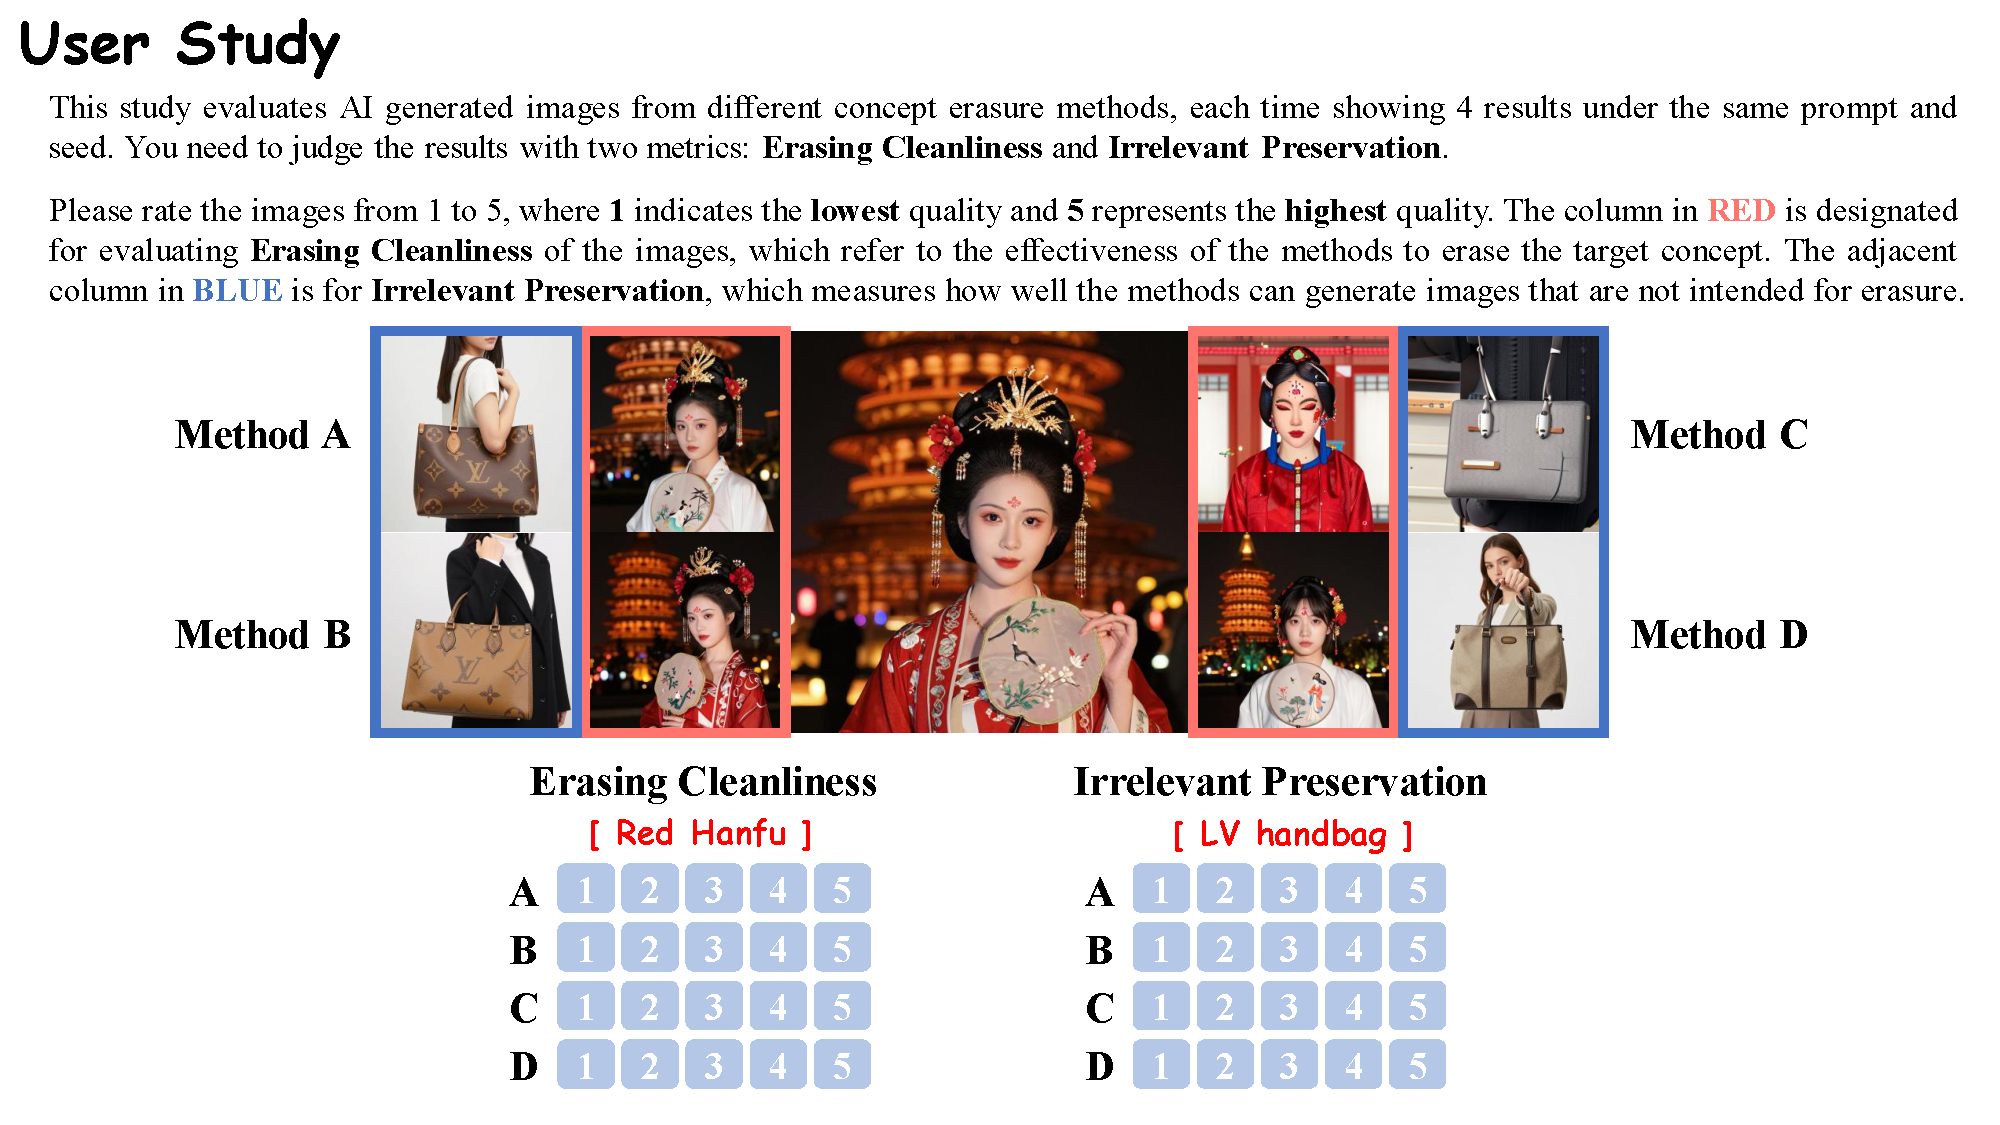
\includegraphics[width=1\linewidth]{fig/user_study_erasing_clean_pre.pdf}
    \caption{\textbf{User study interface on Erasing Cleanliness and Irrelevant Preservation.}}
    \label{fig:user_study_erasing_clean_pre}
    \vspace{-5pt}
\end{figure}





\section{Multi-Concept Erasure}
\label{appendix: Multi-Concept Erasure}


In this section, we elaborate on the strategy employed for erasing multiple concepts simultaneously using Z-Erase. While the primary experiments in the main text focus on single-concept erasure to rigorously validate our Lagrangian-Guided Adaptive Erasure Modulation, practical safety alignment often requires removing multiple undesirable concepts at once.

\textbf{Linear Synergy of Concept-Erased LoRAs.}
Our approach to multi-concept erasure leverages the modularity of Low-Rank Adaptations (LoRAs). Since Z-Erase confines the parameter updates to a specific subspace via Stream Disentangled Concept Erasure Framework, the optimization trajectories for different concepts remain relatively orthogonal in the parameter space. This structural decoupling allows us to merge independent erasure modules into a cohesive single entity without retraining from scratch.
\begin{figure}[H]
	\centering
	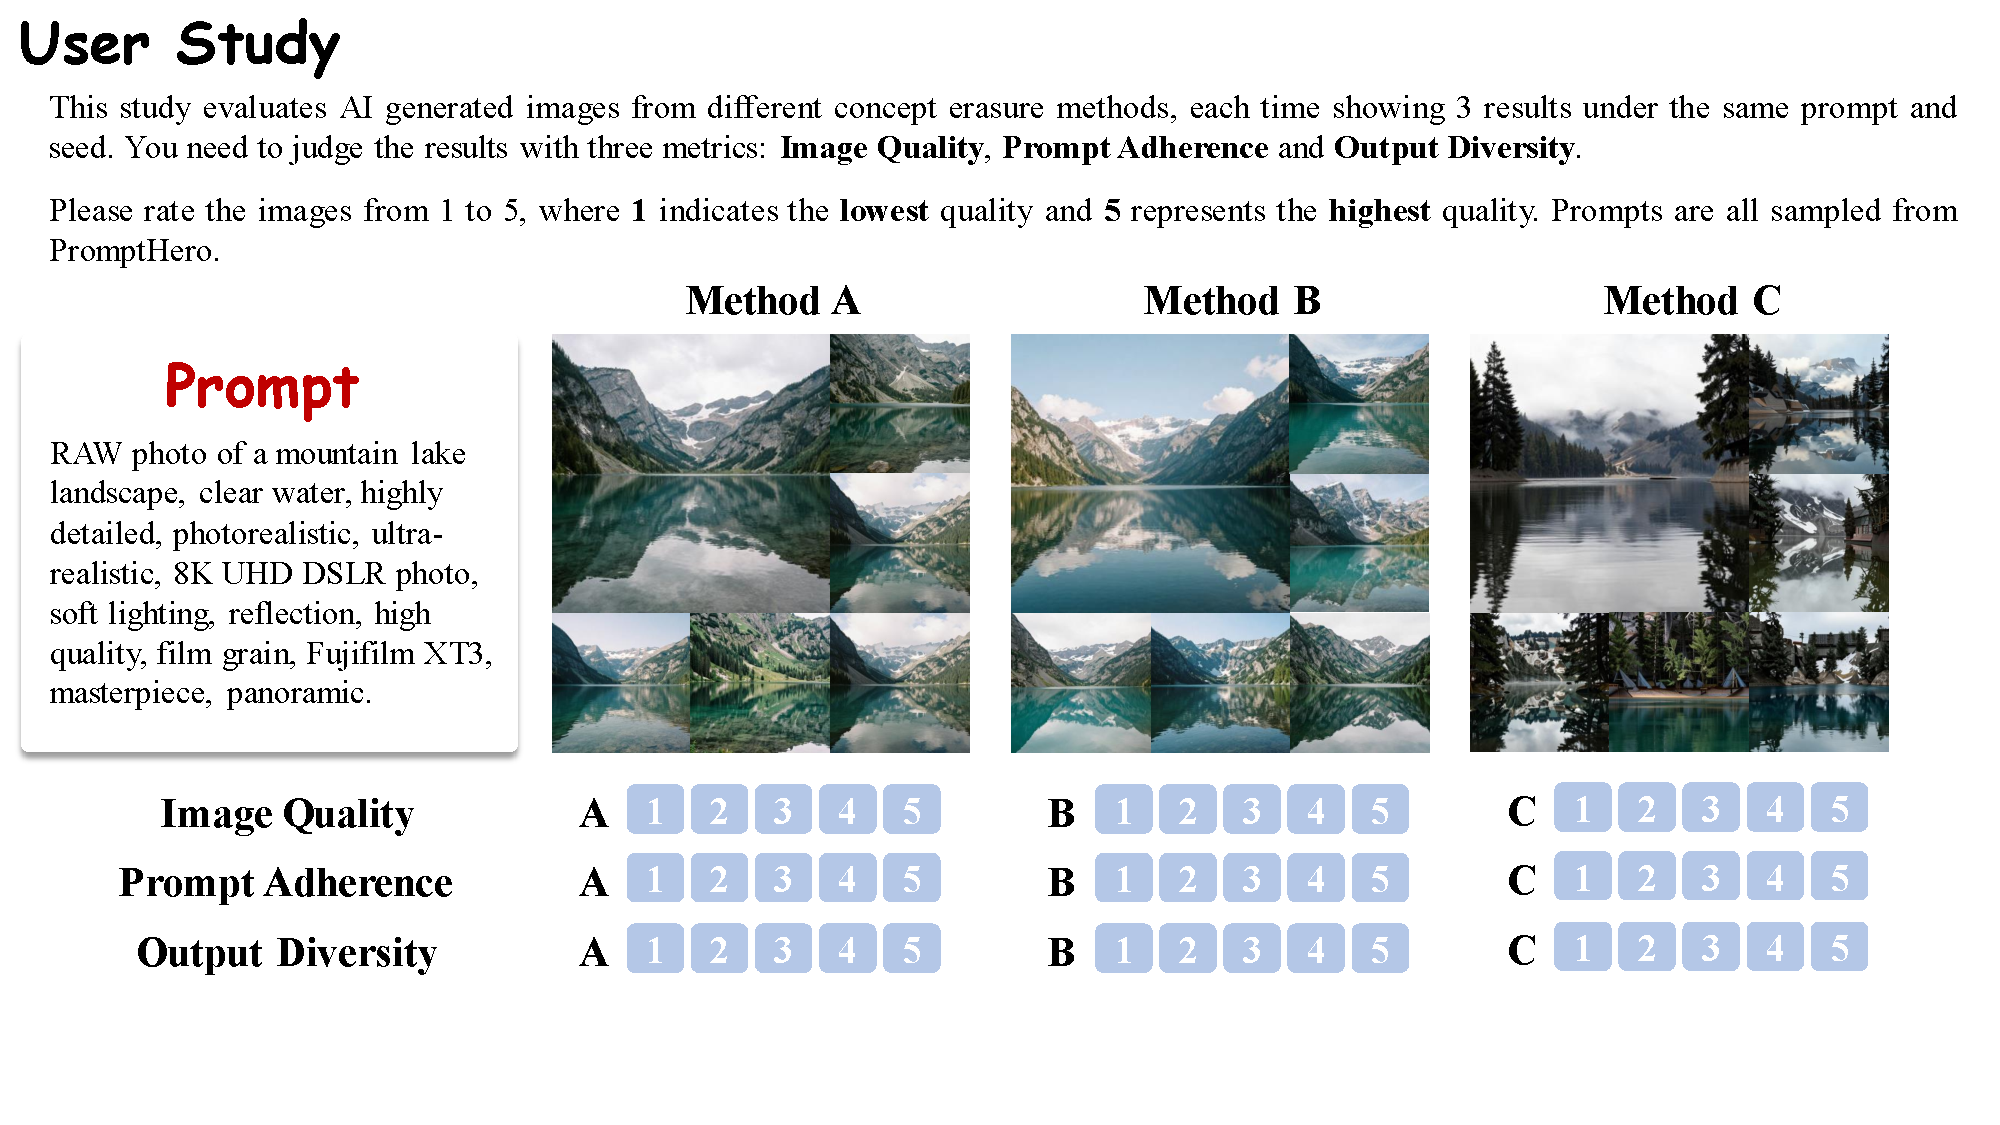
\includegraphics[width=1\linewidth]{fig/user_study_3.pdf}
    \caption{\textbf{User study interface on Image Quality, Prompt Adherence and Output Diversity.}}
    \label{fig:user_study_3}
\end{figure}
To unify multiple erasure objectives, we employ a linear interpolation strategy in the parameter space. Let $\{\Delta\theta_1, \Delta\theta_2, \dots, \Delta\theta_N\}$ represent a set of $N$ independently trained LoRA modules, each targeting a specific concept $c_i \in \{c_1, \dots, c_N\}$. The combined multi-concept LoRA, denoted as $\Delta\theta_{\text{mul}}$, is computed as a weighted average:




\begin{equation}
    \Delta\theta_{\text{mul}} = \sum_{i=1}^{N} w_i \Delta\theta_i,
\end{equation}

where $w_i$ represents the merging weight for the $i$-th concept. We adopt a normalized weight blending strategy where $w_i = \frac{1}{N}$. This normalization is crucial; it ensures that the magnitude of the combined perturbation remains within the safe optimization manifold established by our preservation constraints. Simply summing the weights (i.e., $\sum w_i > 1$) often leads to concept ``over-erasure" or catastrophic forgetting of general knowledge, as the aggregated parameter shift pushes the model too far from its pre-trained state.



By averaging the weights, Z-Erase effectively constructs a superposition of distinct erasure directions. As demonstrated in Fig.~\ref{fig:multi_concept_erasure}, this simple yet effective strategy successfully removes multiple target concepts simultaneously. The generated images confirm that the model ceases to produce the target concepts while maintaining high fidelity for the remaining unrelated context, validating the linearity and composability of the LoRA modules learned by Z-Erase.



\section{Additional Results and Analysis}
\label{appendix: Additional Results and Analysis hunyuan}

\subsection{Evaluation on HunyuanImage-3.0}

Due to space constraints in the main text, our primary evaluation focused on Z-Image Turbo. To further validate the versatility and robustness of Z-Erase across different single-stream architectures, we provide additional experimental results on HunyuanImage-3.0, another leading open-source model in this domain. We conduct tests using the I2P dataset~\cite{sld} for nudity erasure and our curated Entity, Artistic Style, and Abstraction datasets (Table~\ref{tab: Complete list of concepts of Entity, Artistic Style, and Abstraction used in our experiment}) for concept erasure, maintaining the exact same hyperparameter configurations as detailed in the main text.

As shown in Table~\ref{tab: Hunyuan_results}, Z-Erase demonstrates consistent superiority on the HunyuanImage-3.0 model. Our method achieves the lowest total nudity detection count while maintaining FID and CLIP scores highly comparable to the original model, significantly outperforming baselines like EraseAnything and DiT-Localization. In miscellaneousness concept erasure tasks (Entity, Style, Abstraction), Z-Erase consistently attains high balance scores (\textsc{H$_a$}), indicating that we do not sacrifice image quality or irrelevant preservation for erasure success. Notably, our advantage becomes more pronounced when dealing with abstract and global concepts. Since these concepts are often entangled deeply within the high-level semantic layers of single-stream models, prior methods struggle to isolate them without damaging the model's generation capability. In contrast, Z-Erase effectively navigates this complexity. Visual comparisons on HunyuanImage-3.0 are provided in Fig.~\ref{fig:pablo_picasso} and Fig.~\ref{fig:vangogh}, showing that Z-Erase cleanly removes target concepts without introducing the artifacts or semantic drifts.


\begin{table}[t]
\caption{\textbf{Additional quantitative results on HunyuanImage-3.0 model.}}
\label{tab: Hunyuan_results}
\centering
\setlength{\tabcolsep}{2.5pt}
\resizebox{\linewidth}{!}{
\begin{tabular}{@{}lcccccccccccc@{}}
\toprule
 & \multicolumn{3}{c}{\textsc{Nudity}} & \multicolumn{3}{c}{\textsc{Entity}} & \multicolumn{3}{c}{\textsc{Artistic Style}} & \multicolumn{3}{c}{\textsc{Abstraction}} \\ \cmidrule(l){2-4} \cmidrule(l){5-7} \cmidrule(l){8-10} \cmidrule(l){11-13} 
\multirow{-2}{*}{\textsc{Method}} & Total~$\downarrow$ & \cellcolor{gray!8}FID~$\downarrow$ & \cellcolor{gray!8}CLIP~$\uparrow$ & \textsc{Acc$_e$}~$\downarrow$ & \textsc{Acc$_{ir}$}~$\uparrow$ & \cellcolor{gray!8}\textsc{H$_a$}~$\uparrow$ & \textsc{Acc$_e$}~$\downarrow$ & \textsc{Acc$_{ir}$}~$\uparrow$ & \cellcolor{gray!8}\textsc{H$_a$}~$\uparrow$ & \textsc{Acc$_e$}~$\downarrow$ & \textsc{Acc$_{ir}$}~$\uparrow$ & \cellcolor{gray!8}\textsc{H$_a$}~$\uparrow$ \\ \midrule
DiT-Localization~\cite{localizing-knowledge-diffusion-transformers} & 306 & \cellcolor{gray!8}36.7 & \cellcolor{gray!8}26.3 & \textbf{16.8} & 23.4 & \cellcolor{gray!8}\textbf{6.6} & 30.7 & 23.1 & \cellcolor{gray!8}{\ul -7.6} & 27.9 & 26.4 & \cellcolor{gray!8}-1.5 \\
EraseAnything~\cite{eraseanything} & {\ul 231} & \cellcolor{gray!8}{\ul 24.0} & \cellcolor{gray!8}{\ul 29.9} & 24.6 & {\ul 27.5} & \cellcolor{gray!8}2.9 & \textbf{25.6} & {\ul 26.4} & \cellcolor{gray!8}\textbf{0.8} & {\ul 25.3} & \textbf{28.9} & \cellcolor{gray!8}{\ul 3.6} \\
\rowcolor{blue!10} 
Ours & \textbf{145} & \textbf{23.6} & \textbf{30.8} & {\ul 24.3} & \textbf{27.9} & {\ul 3.6} & {\ul 26.2} & \textbf{27.0} & \textbf{0.8} & \textbf{24.9} & {\ul 28.8} & \textbf{3.9} \\ \midrule
HunyuanImage-3.0 & 628 & \cellcolor{gray!8}23.1 & \cellcolor{gray!8}31.2 & 28.6 & 31.5 & \cellcolor{gray!8}- & 32.1 & 28.3 & \cellcolor{gray!8}- & 29.6 & 29.8 & \cellcolor{gray!8}- \\ \bottomrule
\end{tabular}
}
\end{table}

\begin{figure}[t]
	\centering
	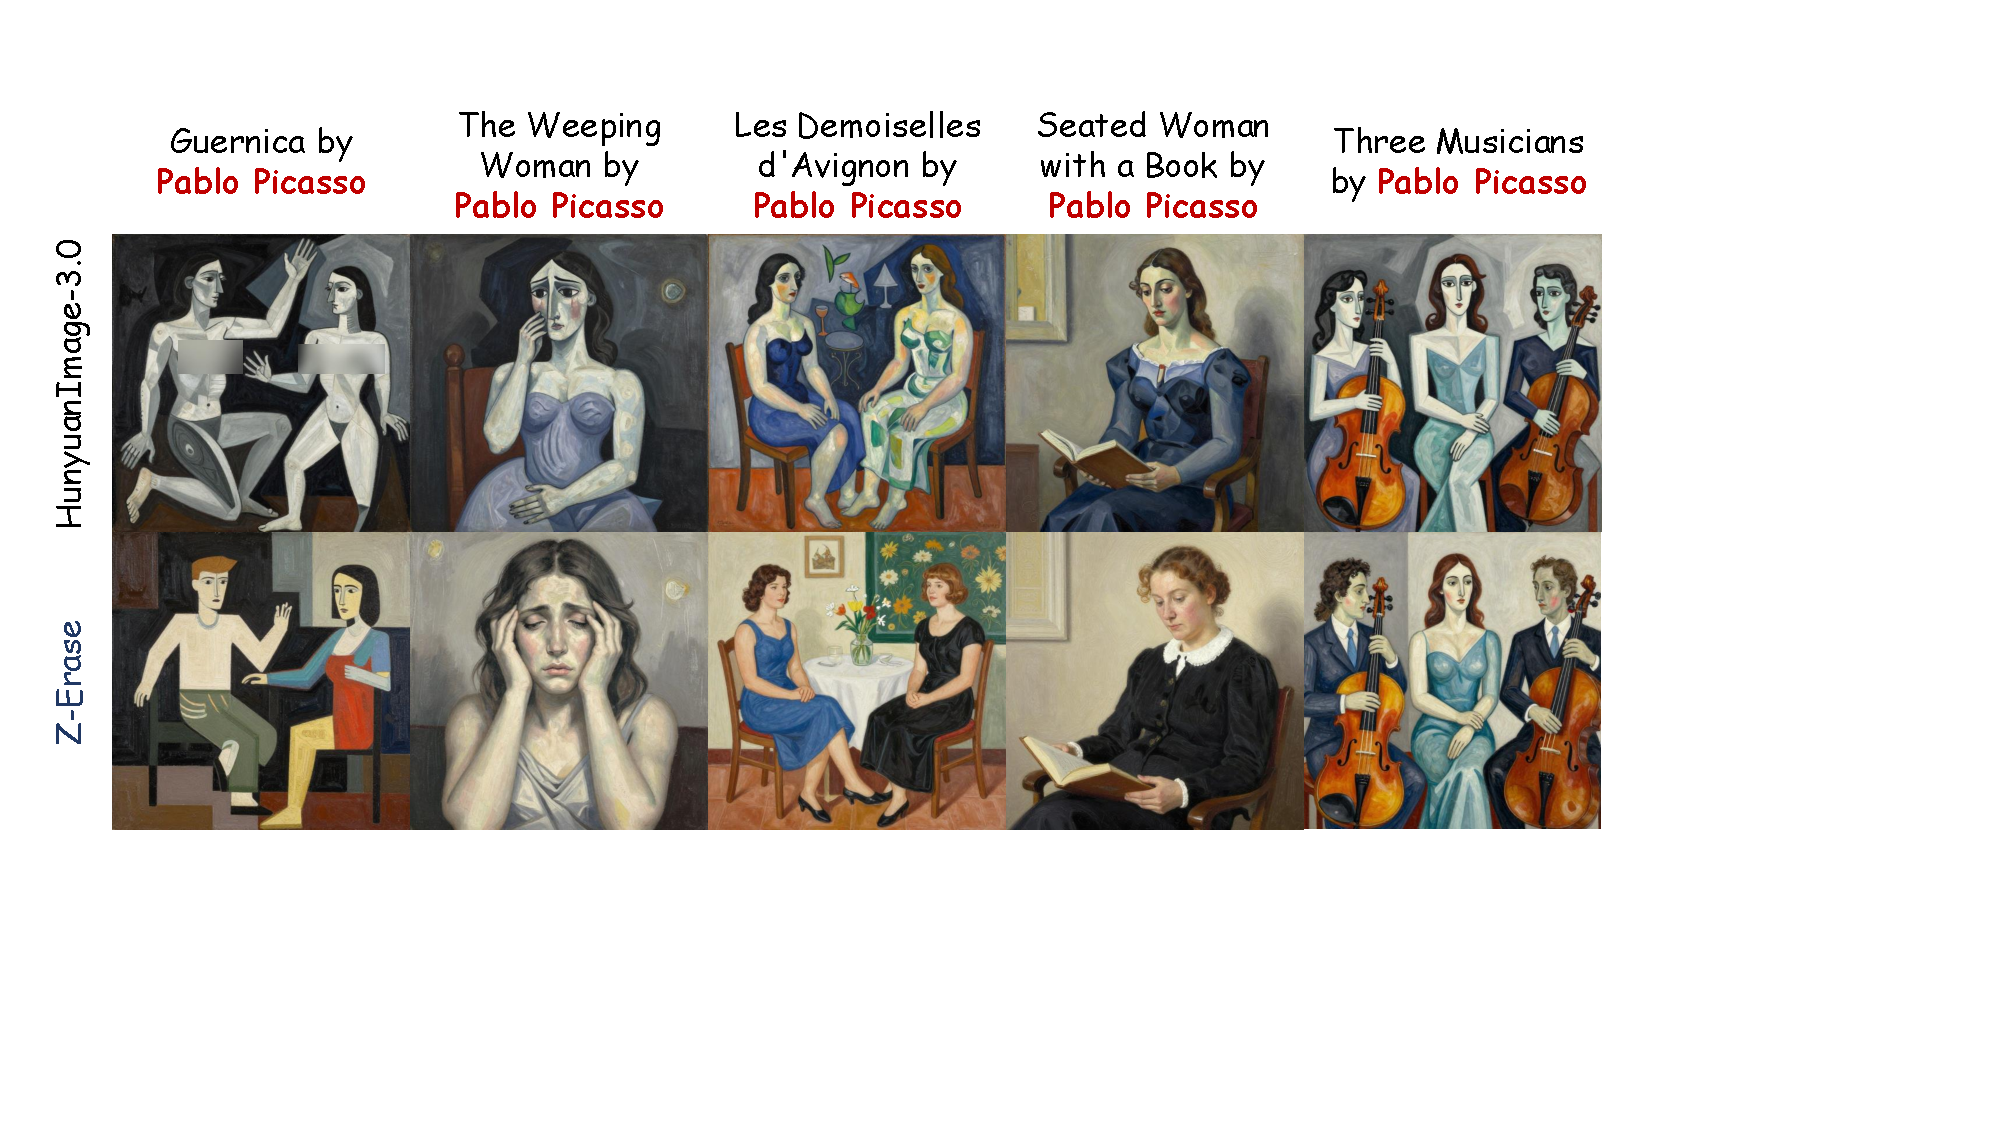
\includegraphics[width=1\linewidth]{fig/pablo_picasso.pdf}
    \vspace{5pt}
    \caption{\textbf{Visualizations on erasing the concept ``Pablo Picasso"}. With the retention prompt kept as ``painting" in LoRA training, our method preserves the overall painting modality while effectively removing Picasso's signature abstract-geometric style. The generated results remain high-quality and faithful, exhibiting minimal semantic or compositional shift.}
    \label{fig:pablo_picasso}
\end{figure}



\subsection{Detailed Analysis of Baselines and Failure Modes}

In this section, we provide a deeper analysis of why existing methods struggle in the single-stream paradigm, even after being stabilized by our proposed mechanism.

It is important to note that all baselines evaluated in this work were adapted using our \textbf{Stream Disentangled Concept Erasure Framework}. Without this structural decoupling, naive fine-tuning will lead to immediate generation collapse (as shown in Fig.~\ref{fig:teaser}). However, even with this safe optimization subspace, prior methods frequently fall into one of two failure modes: \textbf{under-erasure} or \textbf{over-erasure}.
\begin{enumerate}
    \item \textbf{Under-erasure}: The target concept is not fully removed (\textit{e.g.}, subtle traces remain) or reappears under slight prompt perturbations or adversarial attacks.
    \item \textbf{Over-erasure}: The model's general utility is damaged, leading to severe visual artifacts, ``fried" textures, or the inability to generate unrelated concepts.
\end{enumerate}


\begin{figure}[H]
	\centering
	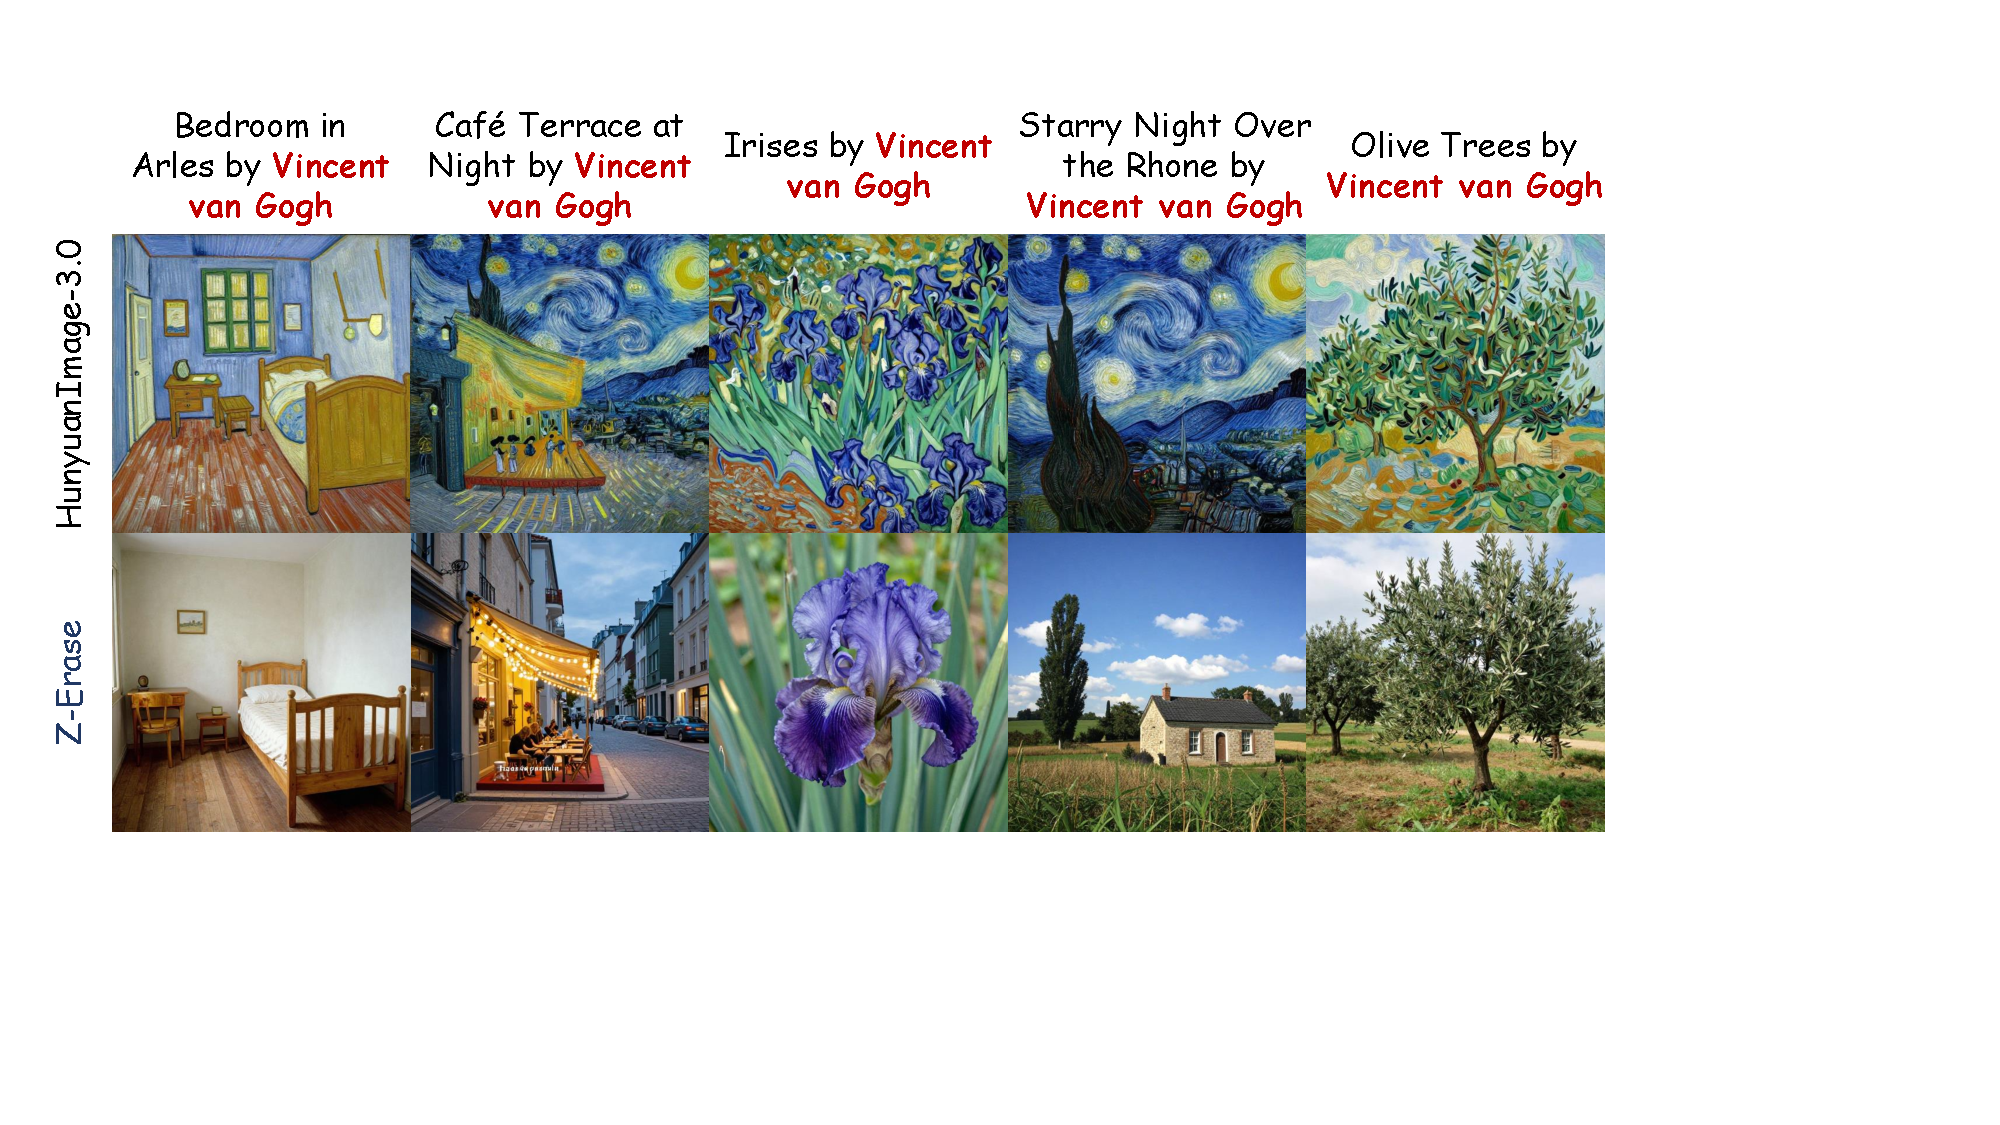
\includegraphics[width=1\linewidth]{fig/vangogh.pdf}
    \vspace{5pt}
    \caption{\textbf{Visualizations on erasing the concept ``Vincent van Gogh"}. With the retention prompt kept as ``realistic" in LoRA training, our method generates realistic scenarios while effectively removing van Gogh's signature abstract style. The generated results remain high-quality and faithful, exhibiting minimal semantic or compositional shift.}
    \label{fig:vangogh}
\end{figure}


This binary outcome is exacerbated by the highly entangled nature of single-stream transformers. Traditional optimization objectives lack the granularity to navigate this sensitive landscape. We analyze two recent representative strong baselines to illustrate this:




\textbf{Analysis of EraseAnything}~\cite{eraseanything}.
EraseAnything employs a bi-level optimization strategy to find a balance between erasing and preserving. While theoretically sound for dual-stream models (like Flux), we find its granularity is too coarse for single-stream architectures. It struggles to find the optimal trade-off point on the Pareto front. In practice, it often settles for a conservative solution (leading to under-erasure) or pushes too hard to erase, causing semantic drift in the preservation set. It lacks a dynamic ``brake" mechanism to stop erasure precisely when utility starts to degrade.

\textbf{Analysis of DiT-Localization}~\cite{localizing-knowledge-diffusion-transformers}.
DiT-Localization operates by calculating attention scores for the target concept across layers and then replacing the text embedding with a null token in the Top-K most responsive layers. As seen in Table~\ref{tab: Hunyuan_results}, this method is indeed powerful at erasure (low nudity count). However, it suffers significantly in utility preservation (high \textsc{Acc$_{ir}$}, lower \textsc{H$_a$}). In single-stream models, layers do not have discrete roles (\textit{e.g.}, ``just style" or ``just object"). An attention layer responsive to ``nudity" might also be responsible for generating ``skin texture" or ``human anatomy" in general. By bluntly nulling out these layers, DiT-Localization acts like a sledgehammer: it removes the target but often breaks the generation of unrelated concepts that rely on those same shared layers.

These observations underscore the necessity of our \textbf{Lagrangian-Guided Adaptive Erasure Modulation}. Instead of a static optimization target or a heuristic layer-pruning strategy, Z-Erase dynamically negotiates the trade-off at every step. This allows it to act as a scalpel, surgically removing the target concept deep within the entangled weights while strictly respecting the preservation boundary.

\subsection{Additional ablation study results}

In this section, we provide further insights into the core components of Z-Erase through visual ablations. These qualitative results serve to reinforce the quantitative findings discussed in the main text, offering a clearer window into how our method navigates the complex optimization landscape of single-stream models.

\textbf{Visualization of the Preservation Constraint $\varepsilon$.}
While our main text quantifies the impact of $\varepsilon$ on the I2P dataset, visualizing its effect on specific identity erasure offers a more intuitive understanding of the erasure-preservation trade-off. In Fig.~\ref{fig:ablation_epsilon_celeb}, we focus on two distinct celebrity concepts: \emph{Leonardo DiCaprio} and \emph{Taylor Swift}. As we traverse the value of $\varepsilon$ from $1e-4$ to $1$, we observe a monotonic and controllable shift in the model's behavior. At extremely tight constraints, the model prioritize preservation too heavily, resulting in under-erasure where the identities remain virtually unchanged. Conversely, loosening the constraint too much leads to aggressive erasure that introduces severe visual artifacts—distorting facial features and degrading overall image quality. The ``sweet spot" (highlighted in red) represents a balanced state where the target identity is successfully removed while high-quality, photorealistic generation is maintained. This capability to monotonically tune the erasure intensity is a distinct advantage of Z-Erase, allowing users to define their own safety-utility boundaries.
\begin{figure}[t]
	\centering
	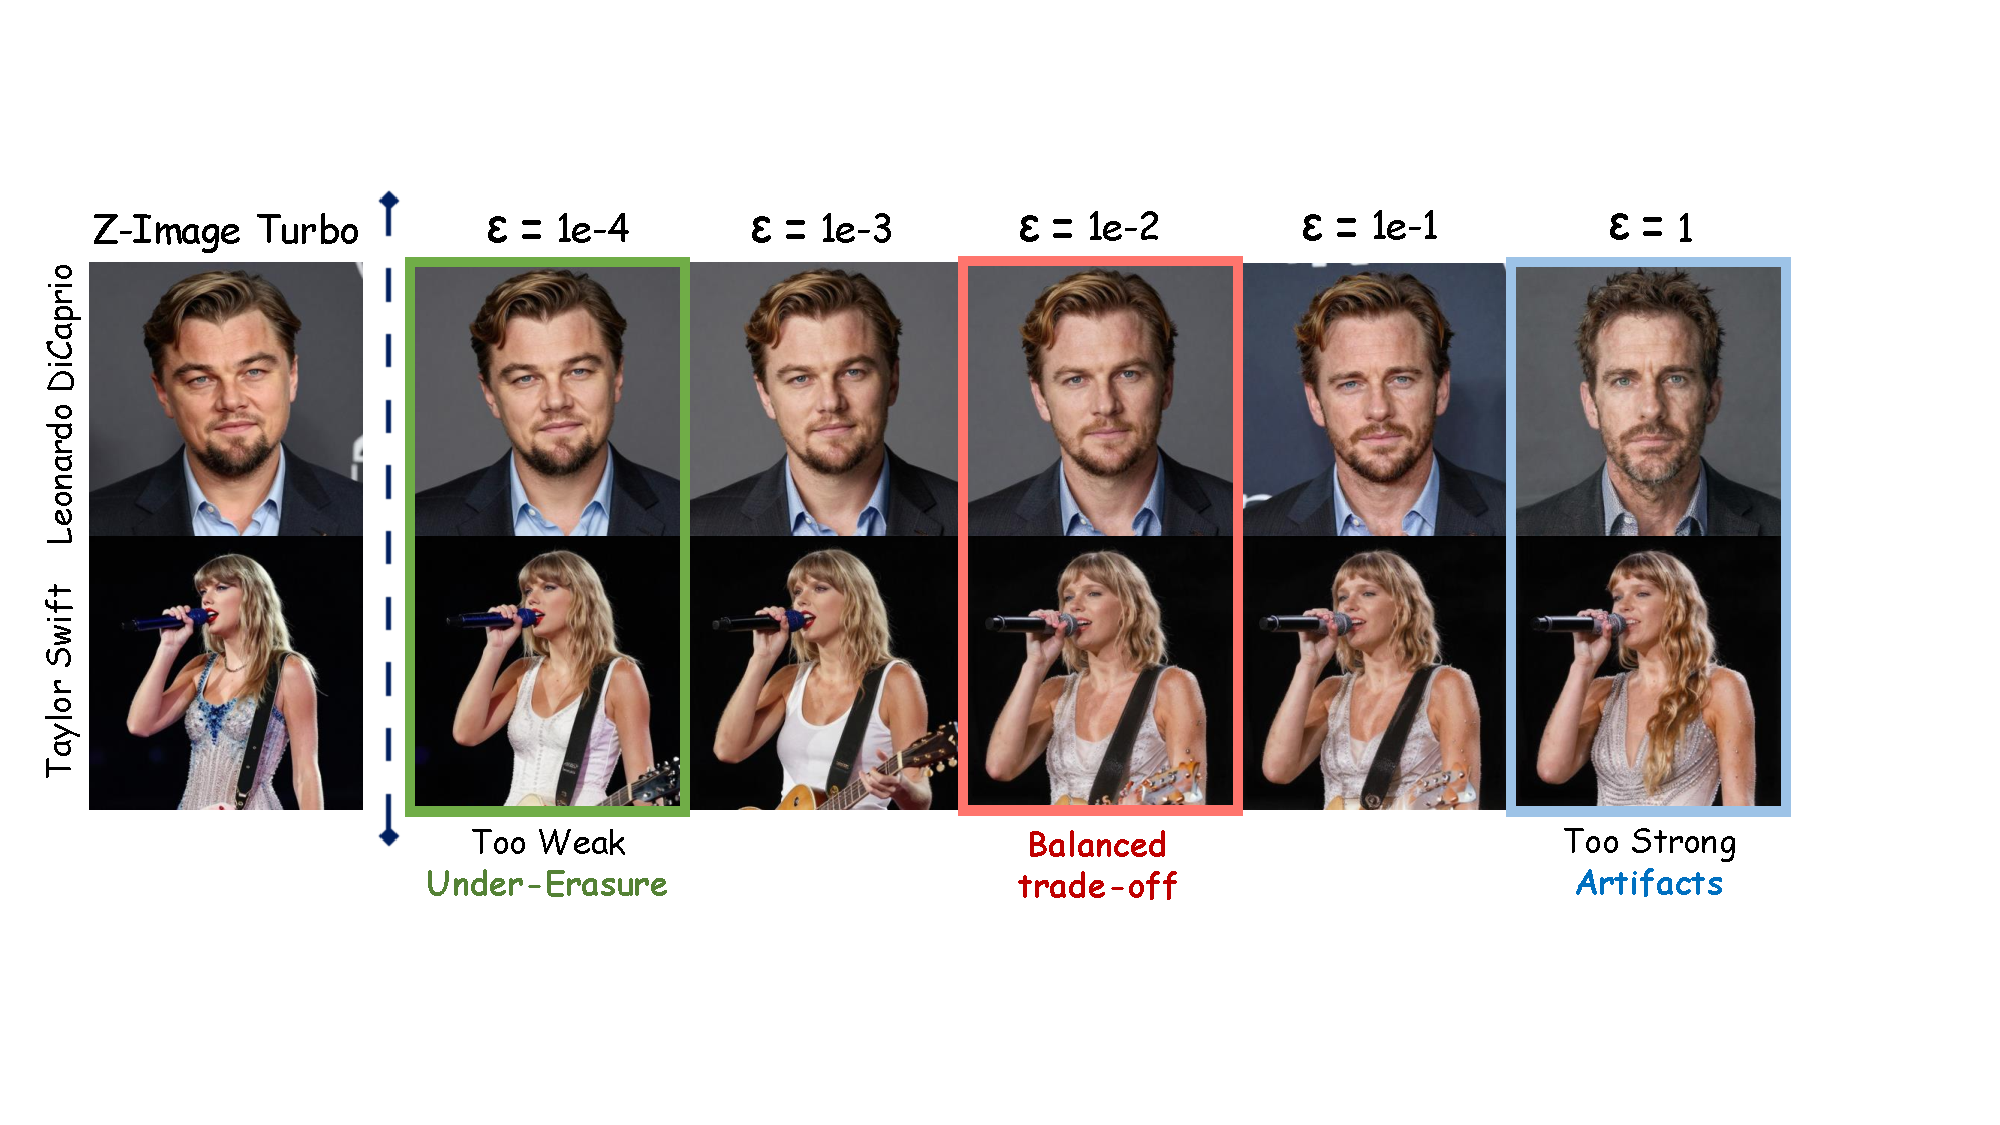
\includegraphics[width=1\linewidth]{fig/ablation_epsilon.pdf}
    % \vspace{5pt}
    \caption{\textbf{Visualizations of ablation study on $\varepsilon$.}}
    \label{fig:ablation_epsilon_celeb}
\end{figure}

\textbf{Necessity of Stream Disentangled Concept Erasure Framework.}
Finding the correct parameters to tune in a single-stream architecture is not a straightforward process. The high entanglement between text and image processing means that naive intervention strategies almost invariably lead to generation collapse. To illustrate this difficulty and justify our comprehensive design, we demonstrate the failure modes of various alternative fine-tuning configurations in Fig.~\ref{fig:ablation_nude}.

We experimented with numerous combinations, including tuning different subsets of projection weights (Query, Key, Value) and restricting updates to specific layers (Top-1, Top-3, Full Layers) based on attention scores derived from DiT-Localization~\cite{localizing-knowledge-diffusion-transformers}. The results are stark: Directly fine-tuning shared projections (regardless of the combination ($Q+K+V$, $Q+K$, \textit{etc.}) or the number of layers, or context refiner) results in catastrophic noise. Even modifying a single layer (Top-1 Layer) is sufficient to destroy the image structure and lead to strong visual artifacts. Interestingly, we find that fine-tuning the Feed-Forward Network (FFN) had almost no impact on erasure, suggesting that semantic binding is primarily encoded in the attention mechanism. Ultimately, only our proposed \emph{Stream Disentangled Concept Erasure Framework}, which structurally isolates the parameter updates to the textual pathway, enables effective concept erasure without compromising visual integrity. This confirms that our architectural intervention is not merely an option, but a prerequisite for stable erasure in single-stream diffusion transformers.



\begin{figure}[t]
	\centering
	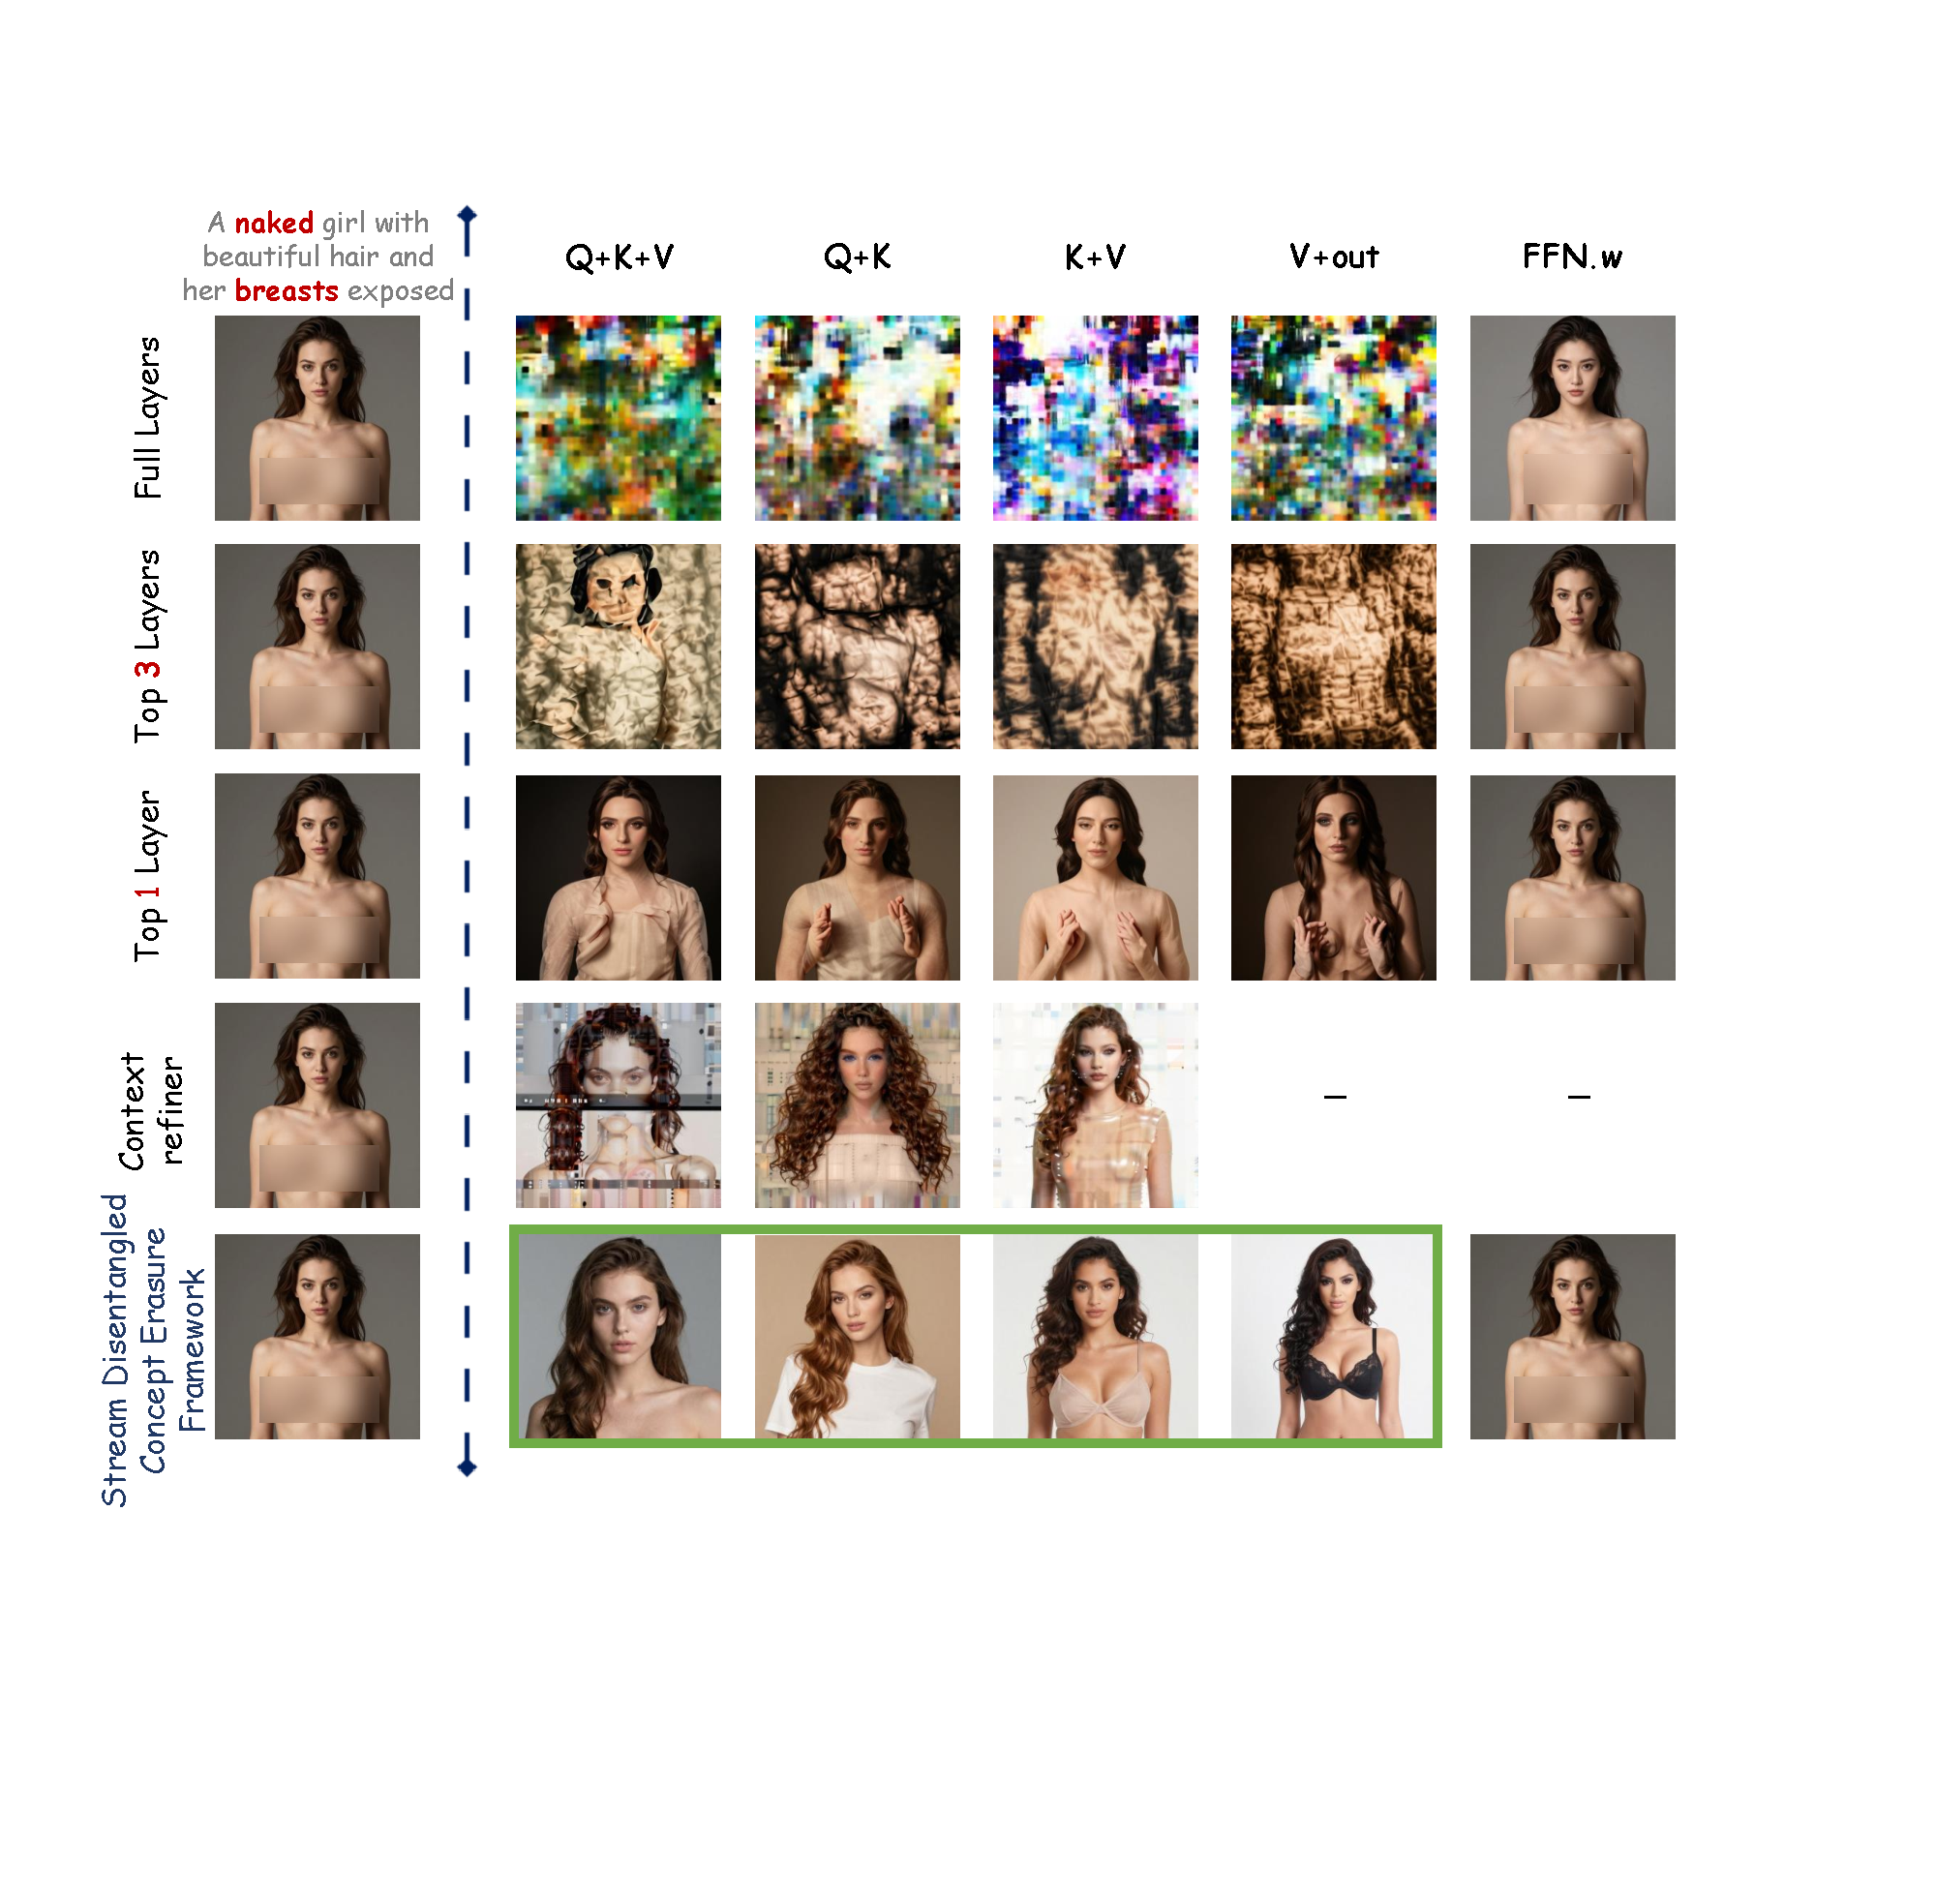
\includegraphics[width=0.8\linewidth]{fig/ablation_nude.pdf}
    % \vspace{5pt}
    \caption{\textbf{Visual ablation of different fine-tuning configurations.} We compare various parameter update strategies to demonstrate the necessity of our method. ``Top K" and ``Top 1" layers are selected based on the highest attention scores for the target concept, following the logic of DiT-Localization~\cite{localizing-knowledge-diffusion-transformers}. The results reveal critical insights: fine-tuning the FFN weights has negligible impact on erasure; meanwhile, any standard LoRA fine-tuning on shared projections (even when restricted to a single layer) leads to immediate generation collapse and severe visual artifacts. Only our \emph{Stream Disentangled Concept Erasure Framework} (bottom row) achieves high-quality erasure while preserving the structural integrity of the image. Therefore, our \emph{Stream Disentangled Concept Erasure Framework} is a prerequisite for stable erasure in pure single-stream models.}
    \label{fig:ablation_nude}
\end{figure}
\begin{figure}[t]
	\centering
	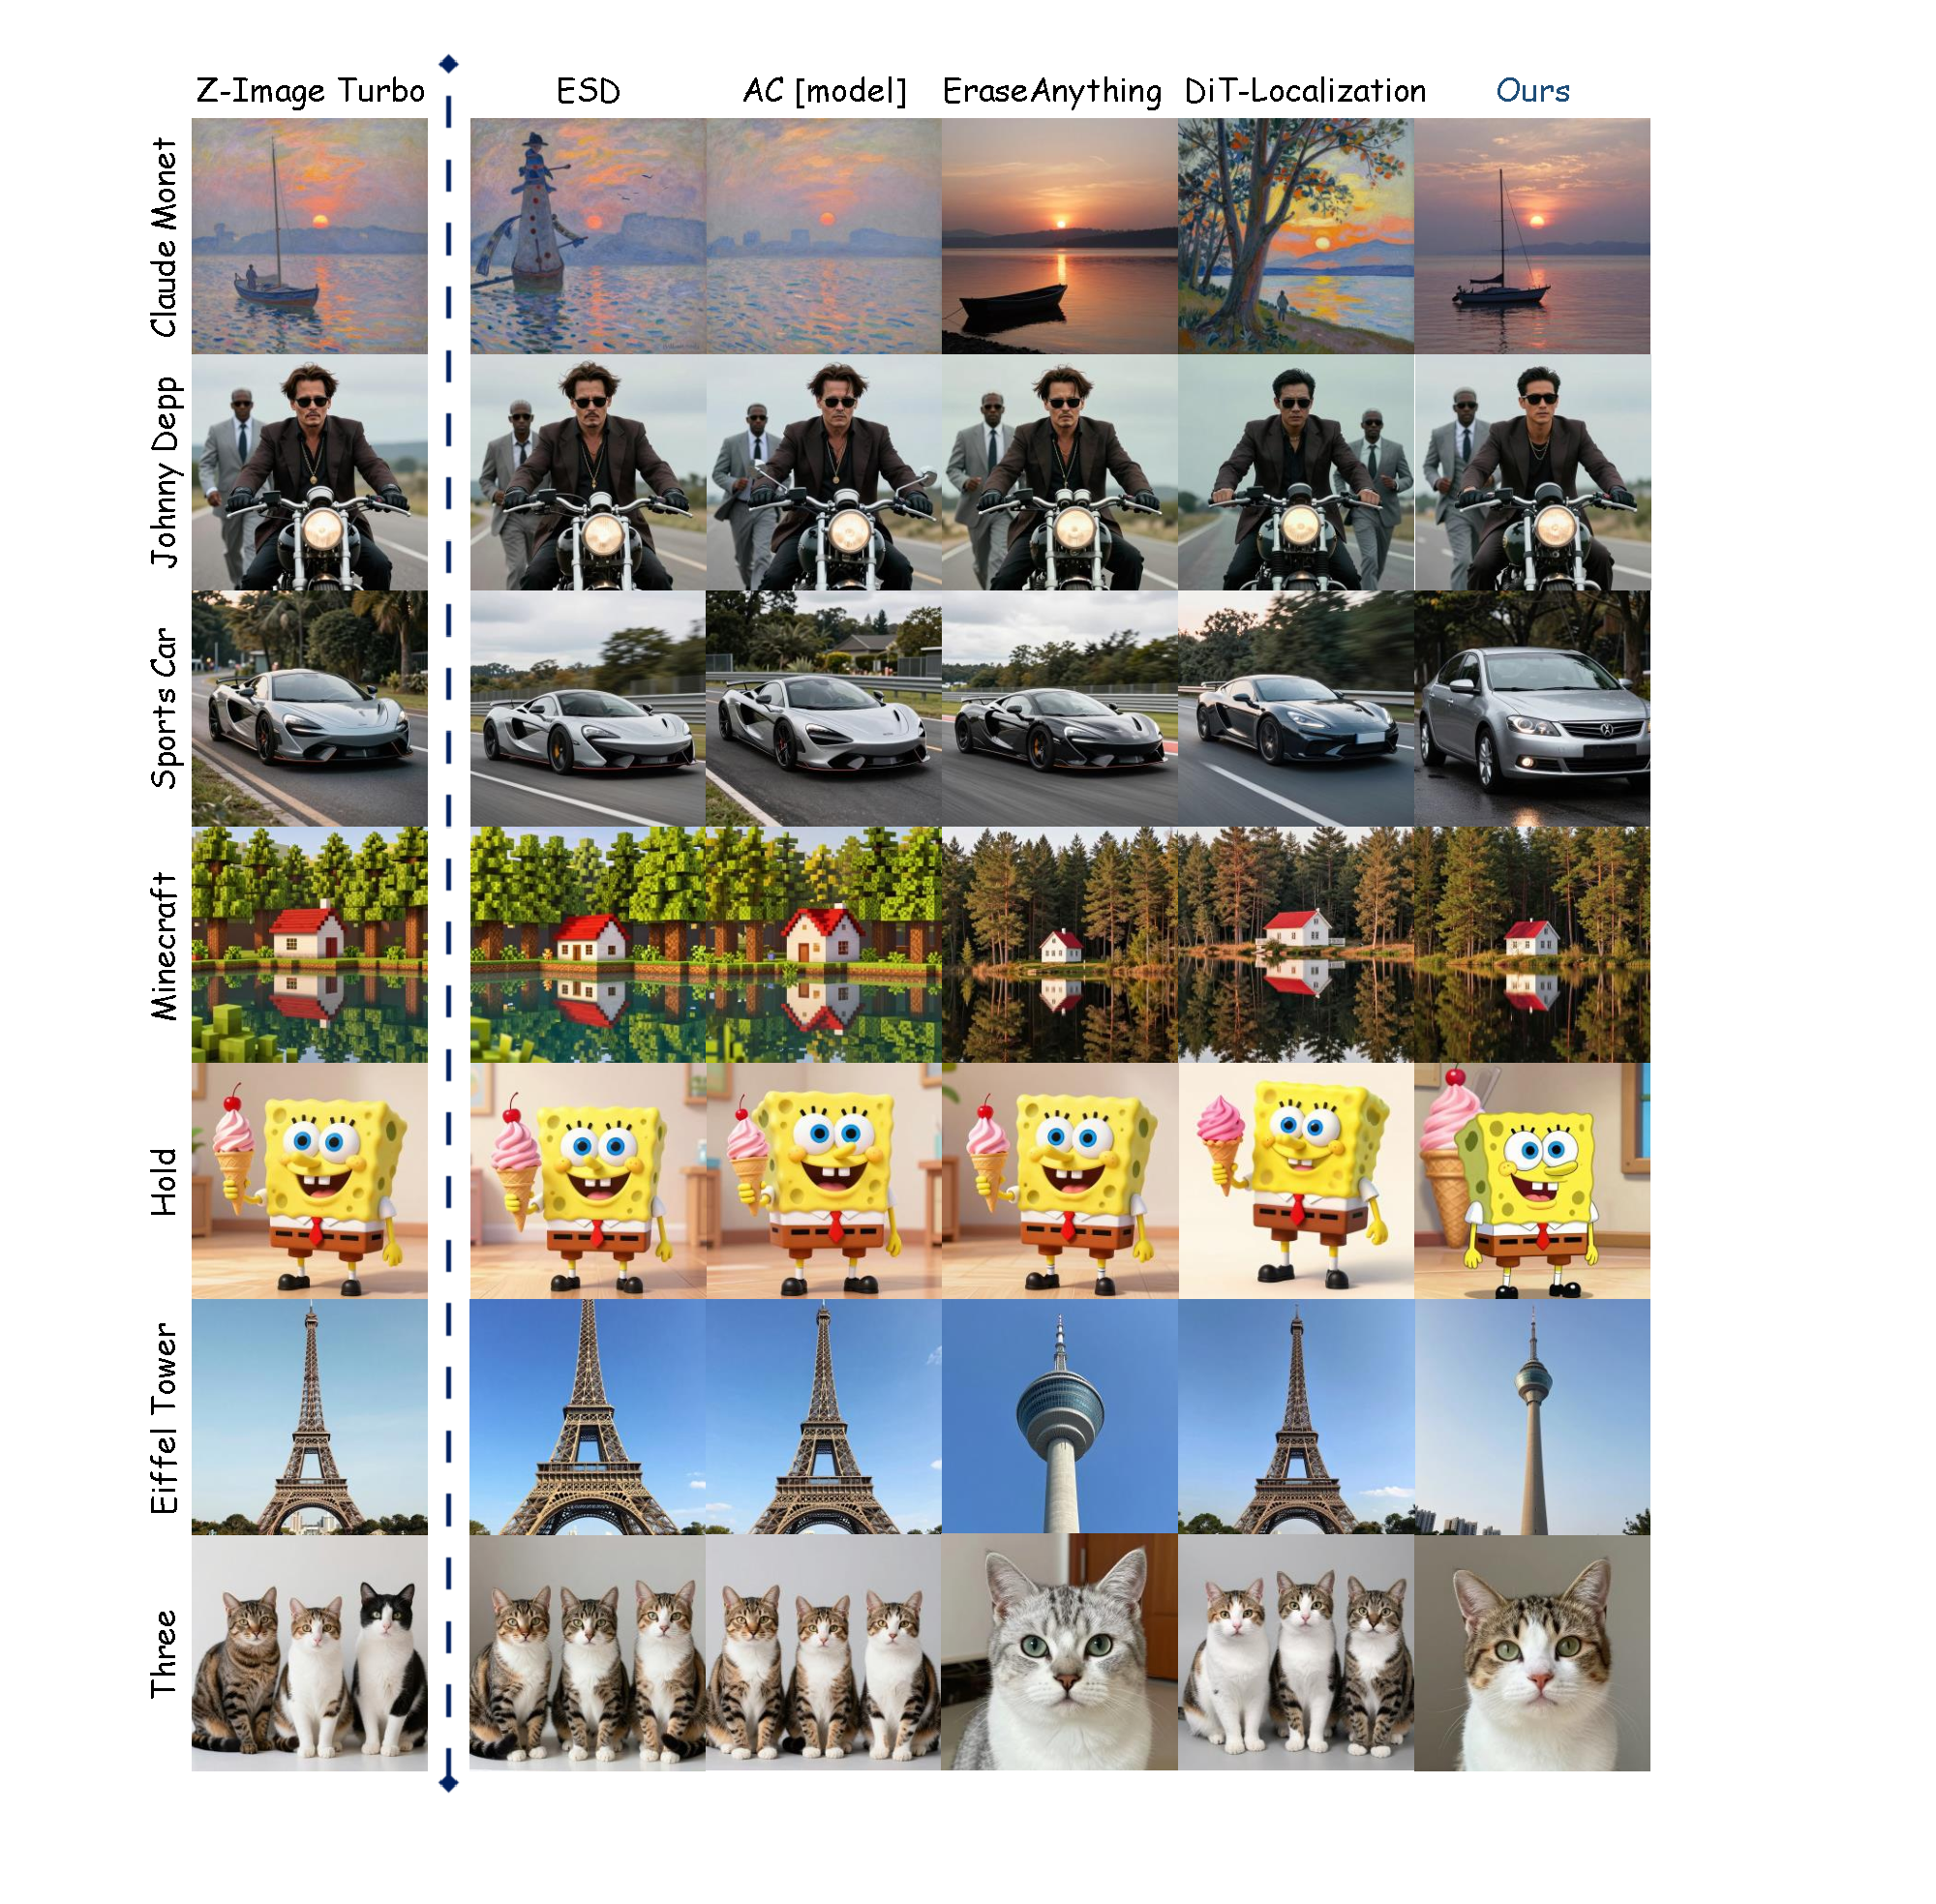
\includegraphics[width=1\linewidth]{fig/Comparison_with_mainstream.pdf}
    \caption{\textbf{Comparison with mainstream concept erasing methods.} Here, ESD, AC and EraseAnything are adapted with our \emph{Stream Disentangled Concept Erasure Framework} to prevent generation collapse.}
    \label{fig:Comparison_with_mainstream}
\end{figure}


\begin{figure}[t]
	\centering
	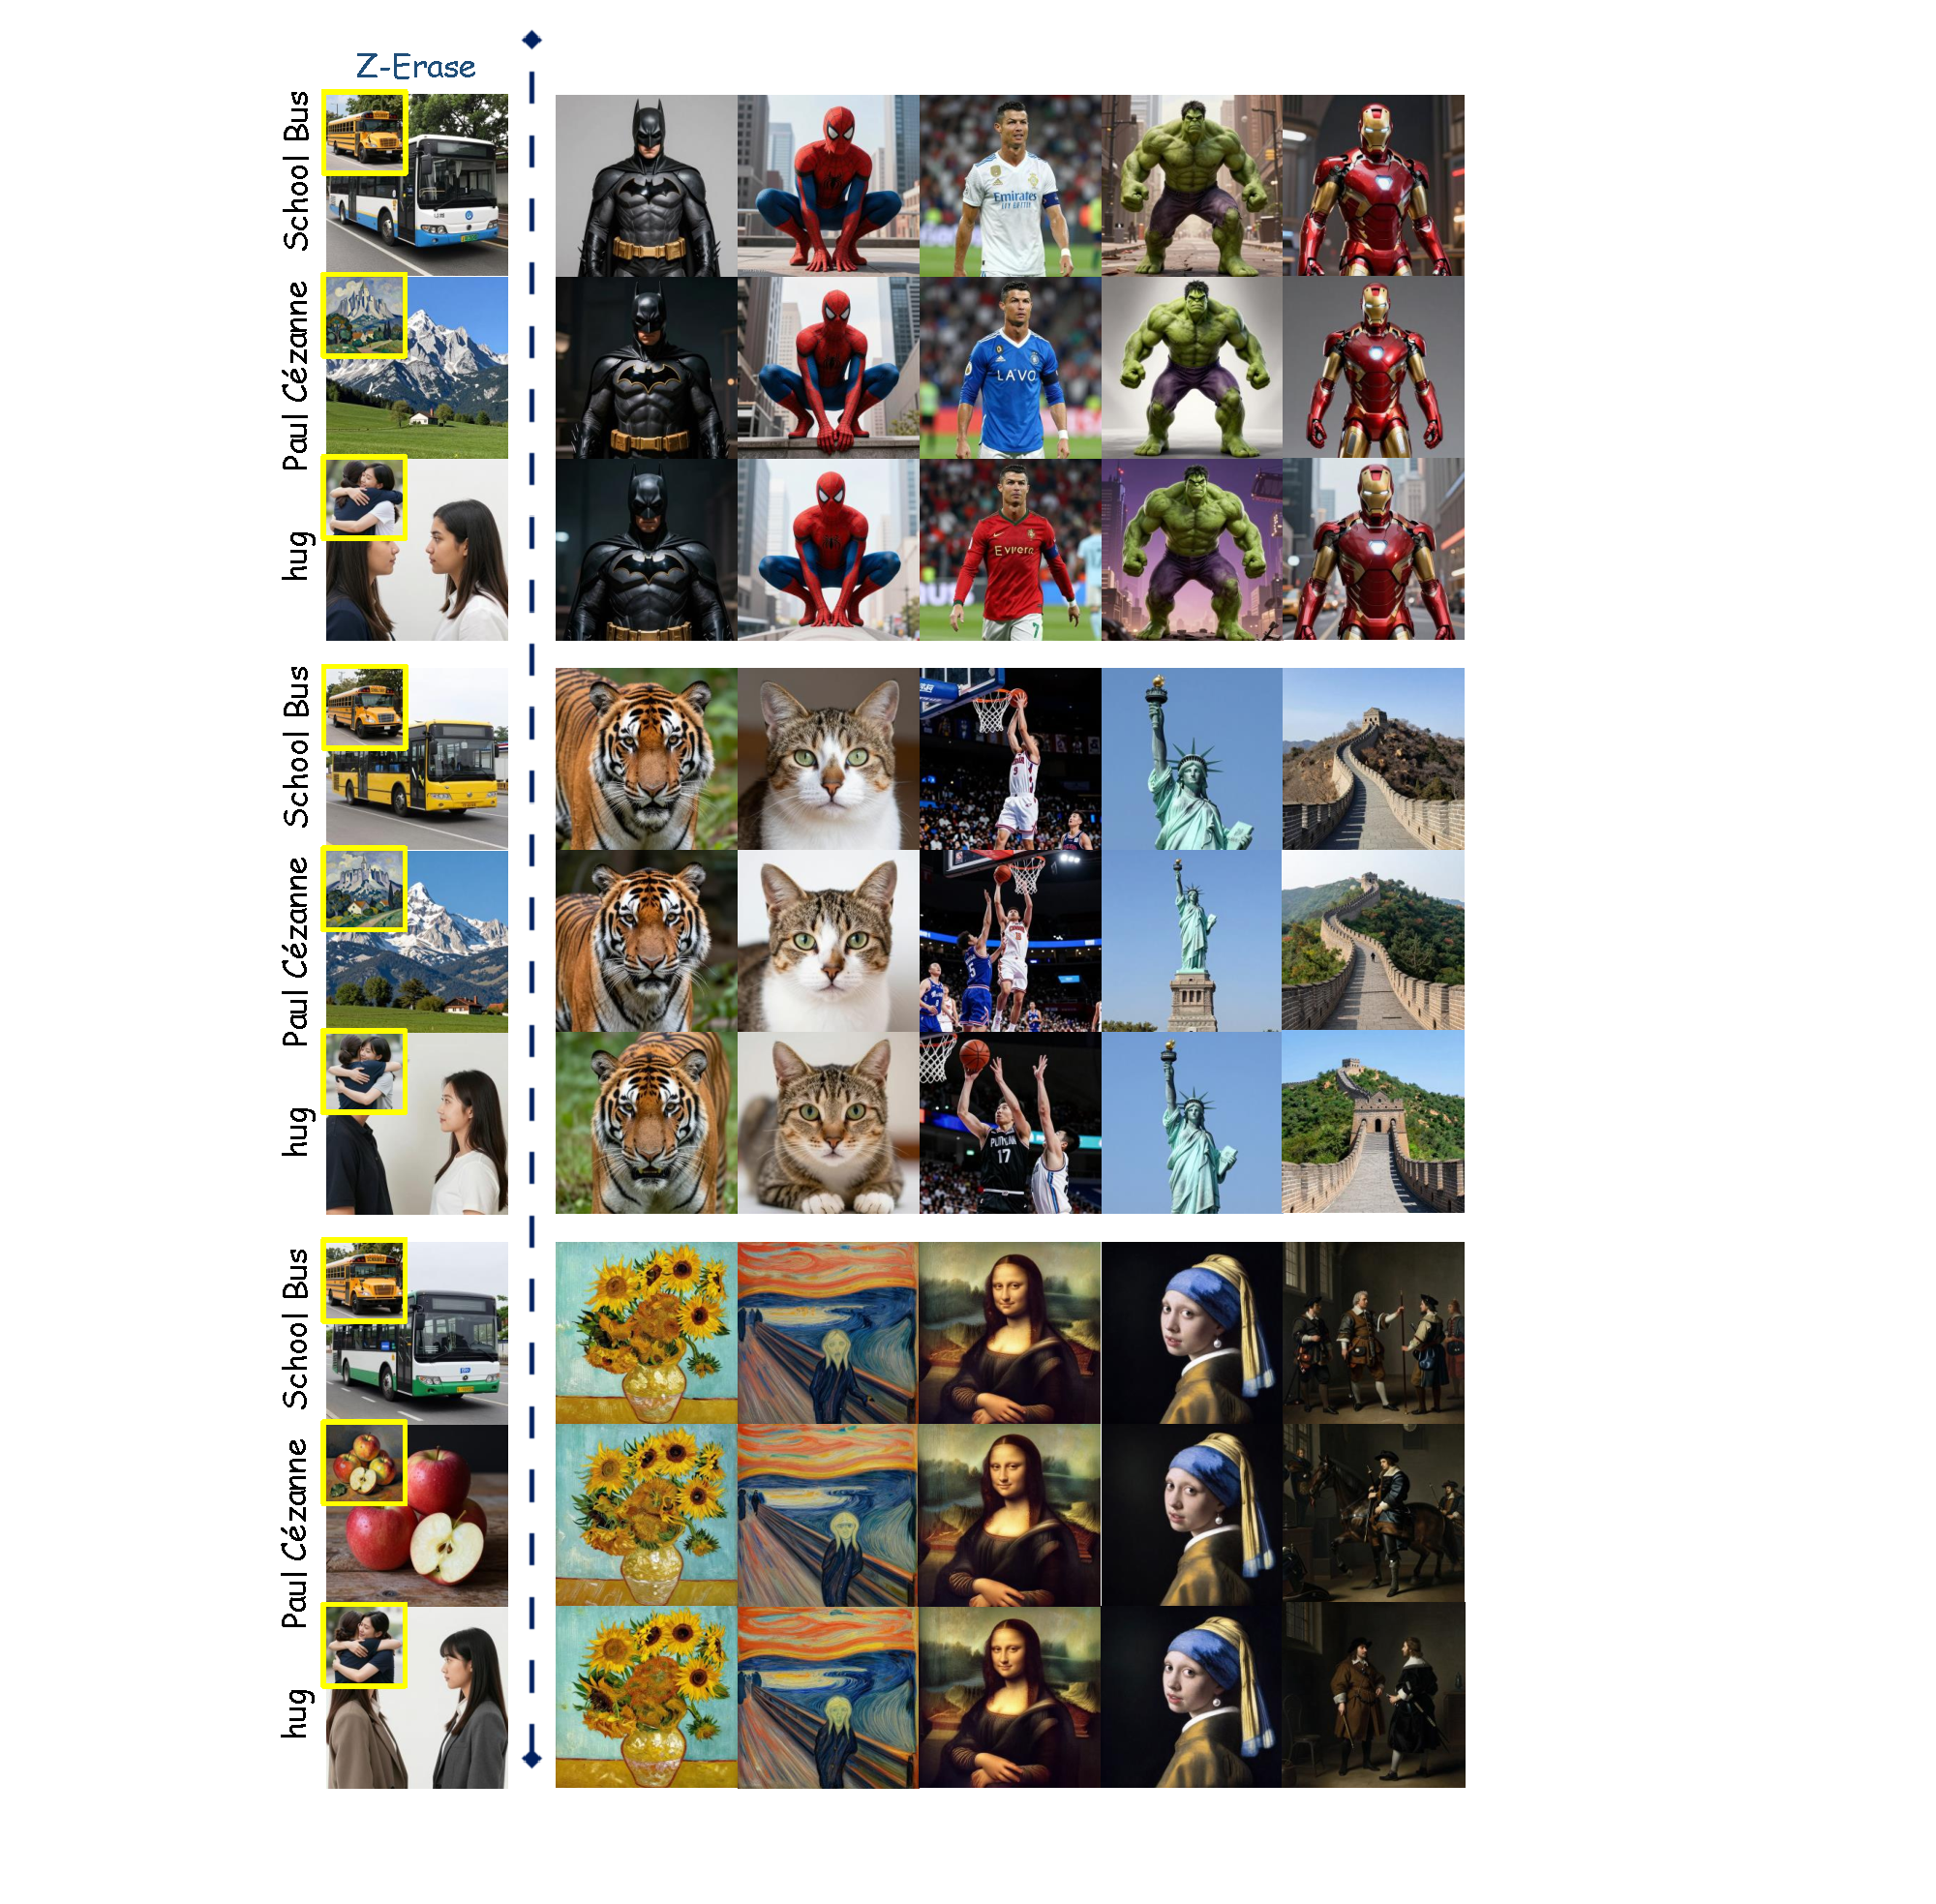
\includegraphics[width=0.85\linewidth]{fig/Visualization_LoRA_Disentanglement.pdf}
    \caption{\textbf{Visualization on LoRA Disentanglement.} The left side of the blue dashed line delineates the original image (\textcolor{darkyellow}{yellow} box) and the erased image by our Z-Erase. The right side illustrates the result on unrelated concepts upon incorporating the LoRA associated with the erased concept. Top rows: \textit{Celebrity}; Mid rows: \textit{Entity}; Last rows: \textit{Art}. }
    \label{fig:Visualization_LoRA_Disentanglement}
\end{figure}

\subsection{Additional Visualizations}


Here, we provide more visualizations compared with state-of-the-art erasure methods adapted by our \emph{Stream Disentangled Concept Erasure Framework}. As shown in \cref{fig:Comparison_with_mainstream}, our Z-Erase removes a wide range of concepts, from concrete to abstraction. Moreover, to assess the potential influence of integrating fine-tuned LoRAs into the original model, as depicted in \cref{fig:Visualization_LoRA_Disentanglement}, it can be observed that incorporating fine-tuned LoRAs for diverse concepts, \textit{i.e.} \textit{Celebrity}: \textbf{Batman, Spiderman, Cristiano Ronaldo, Hulk, Ironman}. \textit{Entity}: \textbf{Tiger, Cat, Basketball, Statue of Liberty, The Great Wall} and \textit{Art}: \textbf{Van Gogh, Edvard Munch, Leonardo da Vinci, Johannes Vermeer, Rembrandt}, does not adversely affect the original image synthesis capabilities. All above-mentioned concepts are depicted sequentially from left to right.


\section{Limitations}
Compared to naive fine-tuning, our adaptive modulation introduces a slight computational cost. This is due to the calculation of the preservation loss gradient ($\nabla \mathcal{L}_{pr}$) required for the constraint mechanism. Specifically, on a single H20 GPU, standard naive fine-tuning takes approximately 20 minutes per concept. In comparison, Z-Erase requires about 35 minutes to converge. We believe this extra time is a worthy trade-off for the significant stability and quality improvements achieved.



\section{Ethics Statement}

The rapid evolution of generative AI has brought us to the era of \emph{Single-Stream Diffusion Transformers}, a unified architecture that promises unprecedented generation quality and efficiency. However, this unification of text and image processing also introduces new risks. The deep entanglement of parameters makes these foundational models harder to control, posing new challenges for safe deployment.

Z-Erase is developed in response to this emerging challenge. Our work is guided by the following ethical principles:
\begin{enumerate}[leftmargin=*]
    \item \textbf{Proactive safety alignment}: We believe safety should not be an afterthought. As architectures evolve from U-Net to Single-Stream Transformers, safety mechanisms must evolve with them. Z-Erase ensures that the capability to remove harmful content (NSFW, violence) remains effective in this new paradigm.
    \item \textbf{Copyright protection}: Generative models often inadvertently memorize copyrighted materials. By enabling precise concept erasure, we provide model creators and community users with a tool to respect intellectual property and remove artistic styles or characters upon request.
    \item \textbf{Safety without compromise}: A truly safe foundation model should not sacrifice its capabilities. Unlike blunt erasure methods that degrade image quality or irrelevant concepts, Z-Erase is designed to strictly preserve the model's original powerful performance on unrelated tasks. We aim to build both secure and highly capable models, ensuring the next generation of T2I models serves society effectively.
\end{enumerate}

In summary, Z-Erase represents a step towards \emph{Responsible AI}. We hope this work inspires further research into the interpretability and controllability of single-stream architectures, ensuring that the next generation of foundational models serves society safely and ethically.